\documentclass[letterpaper,twocolumn,10pt]{article}
\usepackage{usenix}
\usepackage{etoolbox}
\usepackage{xurlshawn}
% \usepackage[hyphenbreaks]{breakurl}

\makeatletter
\patchcmd{\maketitle}
  {\@maketitle}
  {\vspace{-0.3in}\@maketitle\vspace{-0.4in}}% change the value as needed
  {}
  {}
\makeatother

\usepackage{balance}
\usepackage{url}
\usepackage{color}
\usepackage{caption}
\usepackage{diagbox}
\usepackage{subfigure}
\usepackage{mathptmx}
\usepackage{algorithm,algpseudocode}
\usepackage{amsmath,amssymb}

\usepackage{multirow}
\usepackage{booktabs}
\usepackage{epsfig,endnotes}
\usepackage{enumitem}
\usepackage[font=footnotesize,labelfont=bf, labelsep=period]{caption}
\interfootnotelinepenalty=1000
\newcommand{\para}[1]{{\vspace{2pt} \noindent \textbf{#1}
    \hspace{6pt}}}

\newcommand{\subpara}[1]{{\vspace{1.0pt} \textbf{#1}
    \hspace{4pt}}}

\newcommand{\fixme}[1]{{\color{red} #1}}
\newcommand{\todo}[1]{{\color{red}TODO:  #1}}

\newcommand{\askben}[1]{{\color{red} Q:  #1}}
\newcommand{\emily}[1]{{\color{teal} #1}}

\newcommand{\shawn}[1]{{\color{black} #1}}
\newcommand{\jenna}[1]{{\color{purple} #1}}
\newcommand{\htedit}[1]{{\color{black} #1}}

\newcommand{\outline}[1]{{\color{blue} #1}}
\newcommand{\revise}[1]{{\color{black} #1}}
\newcommand{\ol}[1]{{\color{blue} #1}}
\newcommand{\logic}[1]{{\color{brown}LOGIC: #1}}

\newcommand{\etal}{{\em et al.\ }}
\newcommand{\eg}{{\em e.g.,\ }}
\newcommand{\ie}{{\em i.e.,\ }}

\newcommand{\secspace}{\vspace{-0.1in}}
\newcommand{\secspacesm}{\vspace{0.0in}}

\newcommand{\system}{{\em Glaze}}
\newcommand{\dalle}{DALL$\cdot$E-2}
\newcommand{\dalleM}{DALL$\cdot$E-m}
\newcommand\inappendix{\textcolor{blue}{\textbf{in Appendix}}}


\newenvironment{packed_itemize}{
\begin{list}{\labelitemi}{\leftmargin=0.5em}
  \setlength{\itemsep}{1pt}
  \setlength{\parskip}{0pt}
  \setlength{\parsep}{0pt}
  \setlength{\headsep}{0pt}
  \setlength{\topskip}{0pt}
  \setlength{\topmargin}{0pt}
  \setlength{\topsep}{0pt}
  \setlength{\partopsep}{0pt}
}{\end{list}}

\newenvironment{packed_enumerate}{
\begin{enumerate}
 \setlength{\itemsep}{1pt}
 \setlength{\parskip}{0pt}
 \setlength{\parsep}{0pt}
 \setlength{\headsep}{0pt}
 \setlength{\topskip}{0pt}
 \setlength{\topmargin}{0pt}
 \setlength{\topsep}{0pt}
 \setlength{\partopsep}{0pt}
}{\end{enumerate}}

\pagenumbering{gobble}

\begin{document}


\title{Glaze: Protecting Artists from Style Mimicry by Text-to-Image Models}

\author{Shawn Shan, Jenna Cryan, Emily Wenger, Haitao Zheng, Rana Hanocka, Ben Y. Zhao\\
	{\em Department of Computer Science, University of Chicago}\\
	{\em \{shawnshan, jennacryan, ewillson, htzheng, ranahanocka, ravenben\}@cs.uchicago.edu}}
\maketitle


\begin{abstract}
  Recent text-to-image diffusion models such as MidJourney and Stable
  Diffusion threaten to displace many in the professional artist
  community. In particular, models can learn to mimic the artistic style of
  specific artists after ``fine-tuning'' on samples of their art. In this
  paper, we describe the design, implementation and evaluation of \system{},
  a tool that enables artists to apply ``style cloaks'' to their art before
  sharing online. These cloaks apply barely perceptible perturbations to
  images, and when used as training data, mislead generative models that try
  to mimic a specific artist. In coordination with the professional artist
  community, we deploy user studies to more than 1000 artists, assessing
  their views of AI art, as well as the efficacy of our tool, its usability
  and tolerability of perturbations, and robustness across different
  scenarios and against adaptive countermeasures. Both surveyed artists and
  empirical CLIP-based scores show that even at low perturbation levels ($p$=0.05),
  \system{} is highly successful at disrupting mimicry under normal
  conditions (>92\%) and against adaptive countermeasures (>85\%).

\end{abstract}

\section{Introduction}
\label{sec:intro}


Transformers, in particular decoder-only models (e.g.\ GPT~\citep{brown2020language}, Llama~\citep{touvron2023llama}) which process input sequences in a causal fashion, are one of the main drivers of modern deep learning's success.
Numerous approaches attempt to approximate the core attention layer to address its efficiency issues~\citep{tay2022efficient}, such as scaling quadratically in sequence length during training and requiring a cache of size linear in sequence length during autoregressive generation.
In parallel, a class of alternative sequence models, structured state-space models (SSMs), have emerged with linear scaling in sequence length during training and constant state size during generation.
They show strong performance on long-range tasks (e.g. S4~\citep{gu2022efficiently}) and recently matched or beat Transformers on language modeling (e.g. Mamba \citep{gu2023mamba}) at small to moderate scale.
However, the development of SSMs have appeared disjoint from the community's collective effort to improve Transformers, such as understanding them theoretically as well as optimizing them on modern hardware.
As a result, it is more difficult to understand and experiment with SSMs compared to Transformers, and it remains challenging to train SSMs as efficiently as Transformers from both an algorithmic and systems perspective.


Our main goal is to develop a rich body of theoretical connections between structured SSMs and variants of attention.
This will allow us to transfer algorithmic and systems optimizations originally developed for Transformers to SSMs, towards the goal of building foundation models that perform better than Transformers while scaling more efficiently in sequence length.
A milestone contribution in this direction was the \textbf{Linear Attention (LA)} framework \citep{katharopoulos2020transformers},
which derived a connection between autoregressive attention and linear RNNs
by showing the equivalence between ``dual forms'' of quadratic kernelized attention and a particular linear recurrence.
This duality allows new capabilities such as the ability to have both efficient parallelizable training and efficient autoregressive inference.
In the same spirit, this paper provides multiple viewpoints connecting linear-complexity SSMs with quadratic-complexity forms to combine the strengths of SSMs and attention.%
\footnote{Technically speaking, these connections only relate to certain flavors of attention; the title of this paper is an homage to \citet{katharopoulos2020transformers} which first showed that ``Transformers are RNNs''.}

\iftoggle{arxiv}{
\begin{wrapfigure}{R}{0.48\linewidth}
  \begin{center}
    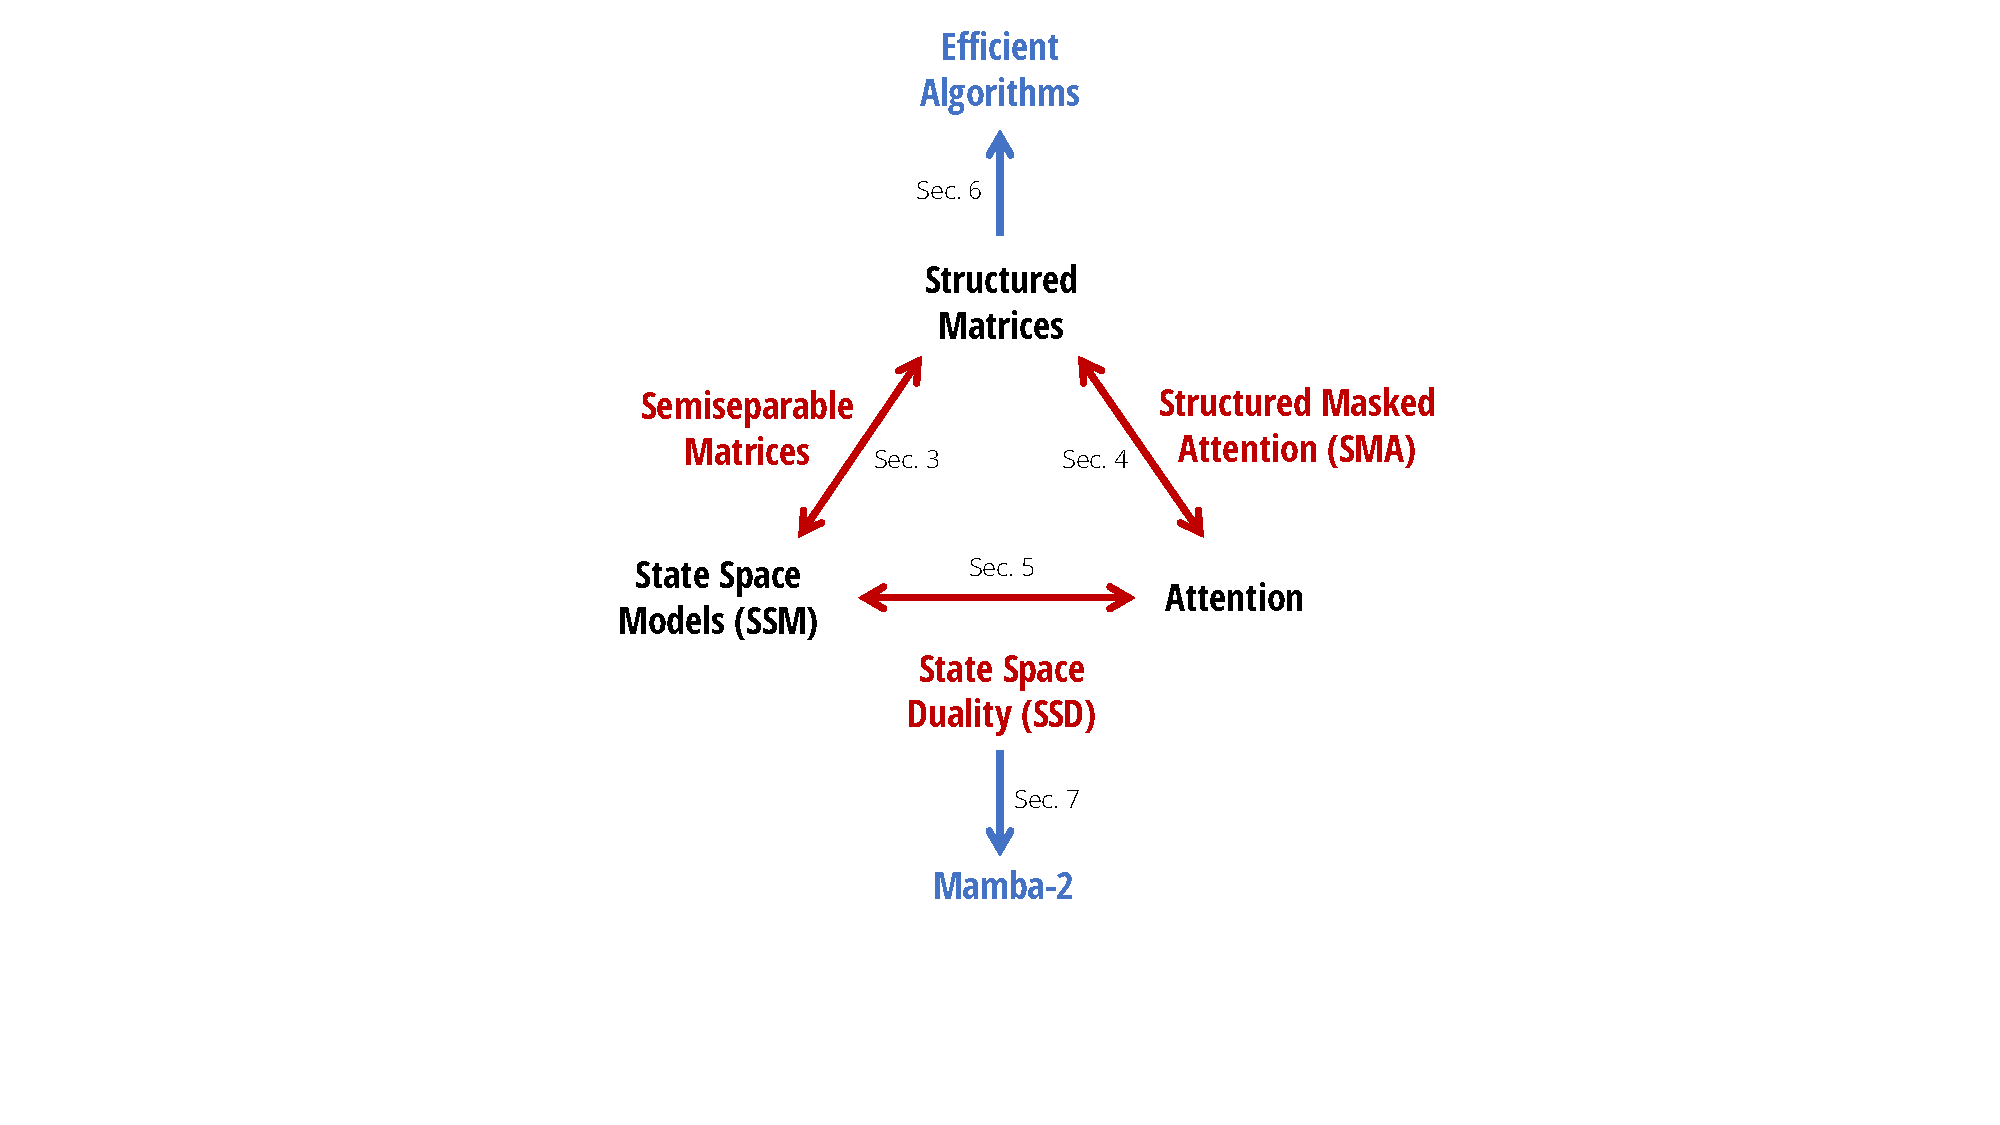
\includegraphics[width=\linewidth]{fig/ssd_roadmap.pdf}
  \end{center}
  \caption{
    (\textbf{Structured State-Space Duality}.)
    This paper fleshes out the relationship between state space models and attention through the bridge of structured matrices.
  }
  \label{fig:roadmap}
\end{wrapfigure}
}{}

\para{State Space Duality.}
Our framework connecting structured SSMs and variants of attention, which we call \textbf{structured state space duality} (SSD),
is made through the abstractions of \textbf{structured matrices}:
matrices with subquadratic parameters and multiplication complexity.
We develop two broad frameworks for representing sequence models, one as matrix transformations and one as tensor contractions, which each reveal different perspectives of the duality.
Our technical contributions include:
\begin{itemize}[leftmargin=*,itemsep=0pt,topsep=0pt]
  \item We show an equivalence between state space models and a well-studied family of structured matrices called \textbf{semiseparable matrices}\iftoggle{arxiv}{ (\cref{sec:ssm})}{}.
    This connection is at the heart our framework, revealing new properties and algorithms for SSMs. A central message of this paper is that \emph{different methods of computing state space models can be reframed as various matrix multiplication algorithms on structured matrices}.
  \item We significantly improve the theory of linear attention~\citep{katharopoulos2020transformers}.
    We first provide an incisive proof of its recurrent form through the language of tensor contractions, and then generalize it to a new family of \textbf{structured masked attention (SMA)}\iftoggle{arxiv}{ (\cref{sec:attention})}{}.
  \item We connect SSMs and SMA, showing that they have a large intersection that are duals of each other, possessing both SSM-like linear and attention-like quadratic forms\iftoggle{arxiv}{ (\cref{sec:ssd})}{}.
    \iftoggle{arxiv}{We also prove that any kernel attention method possessing a fast recurrent form must be an SSM.}{}
\end{itemize}


Beyond its intrinsic theoretical value, our framework opens up a broad set of directions for understanding and improving sequence models.

\para{Efficient Algorithms.}
First and most importantly, our framework exposes new efficient and easily-implementable algorithms for computing SSMs\iftoggle{arxiv}{ (\cref{sec:efficient})}{}.
We introduce a new \textbf{SSD algorithm}, based on block decompositions of semiseparable matrices, that takes advantage of both the linear SSM recurrence and quadratic dual form, obtaining optimal tradeoffs on all main efficiency axes (e.g. training and inference compute, memory usage, and ability to leverage matrix multiplication units on modern hardware).
A dedicated implementation of SSD is $2-8\times$ faster than the optimized selective scan implementation of Mamba, while simultaneously allowing for much larger recurrent state sizes ($8\times$ the size of Mamba or even higher, with minimal slowdown).
SSD is highly competitive with optimized implementations of softmax attention (FlashAttention-2~\citep{dao2023flashattention2}), crossing over at sequence length 2K and 6$\times$ faster at sequence length 16K.


\iftoggle{arxiv}{
\para{Architecture Design.}
One major obstacle to adopting new architectures such as SSMs is the ecosystem tailored to Transformers, such as hardware-efficient optimization and parallelism techniques for large-scale training.
Our framework allows using established conventions and techniques for attention to build a vocabulary of architecture design choices for SSMs, and further improve them (\cref{sec:architecture}).
For example, we introduce the analog of heads from multi-head attention (MHA) to SSMs.
We show that the Mamba architecture is a \textbf{multi-input SSM (MIS)} that turns out to be analogous to \textbf{multi-value attention (MVA)}, and compare other variants of Mamba with different head structures.

We also use these ideas to make slight modifications to the Mamba block, which allows tensor parallelism to be implemented (e.g. in the style of Megatron~\citep{shoeybi2019megatron}).
The main ideas include introducing grouped-value attention (GVA) head structure, and moving all data-dependent projections to occur in parallel at the beginning of the block.


}{
  \para{Mamba-2.}
  Additionally, inspired by the connection between SSMs and Transformers, we slightly modify the neural network architecture of Mamba by moving all data-dependent projections to occur in parallel at the beginning of the block. %
}
The combination of the modified parallel Mamba block, together with using SSD as the inner SSM layer, results in the \textbf{Mamba-2} architecture.
We investigate Chinchilla scaling laws for Mamba-2 in the same setting as Mamba, finding that it Pareto dominates Mamba and Transformer++ in both perplexity and wall-clock time.
We additionally train a family of Mamba-2 models at varying sizes on the Pile, showing that it matches or outperforms Mamba and open source Transformers on standard downstream evaluations.
For example, Mamba-2 with 2.7B parameters trained on 300B tokens on the Pile outperforms Mamba-2.8B, Pythia-2.8B and even Pythia-6.9B trained on the same dataset.

\iftoggle{arxiv}{
\paragraph{Systems Optimizations.}
The SSD framework connects SSMs and Transformers, allowing us to leverage a rich body of work on systems optimizations developed for Transformers~(\cref{sec:systems}).
\begin{itemize}[leftmargin=*,itemsep=0pt,topsep=0pt]
  \item For example, Tensor Parallelism (TP) is an important model parallelism technique to train large Transformer models by splitting each layer across GPUs on the same node.
    We design Mamba-2 to be TP-friendly, reducing the number of synchronization point per block by half.
  \item For very long sequences whose activations do not fit on one device, sequence parallelism has been developed for the attention blocks.
    We describe how to train SSMs in general and Mamba-2 in particular with sequence parallelism, by passing the recurrent states between devices.
  \item For finetuning with examples of different lengths, for best efficiency, Transformer requires sophisticated techniques to remove padding tokens and perform attention on variable length sequences.
    We show how Mamba-2 can be trained with variable sequence lengths efficiently, requiring no padding tokens.
\end{itemize}
}{}

\cref{sec:experiments} empirically validates Mamba-2 on language modeling, training efficiency, and a difficult multi-query associative recall task~\citep{arora2024simple}.
Finally, in \cref{sec:related}, we provide an extended related work and discuss potential research directions opened up by our framework.

Model code and pre-trained checkpoints are open-sourced at \url{https://github.com/state-spaces/mamba}.






\secspace
\section{Background: AI Art and Style Mimicry}
\label{sec:motivation}

In this section, we provide critical context in the form of
basic background on current AI art models and style mimicry.

\secspace
\subsection{Text-to-Image Generation}

Since Text-to-image generation was first proposed in
2015~\cite{mansimov2015generating}, a stream of research has proposed newer
model architectures and training methods enabling generation of
higher-quality
images~\cite{radford2015unsupervised,zhang2017stackgan,xu2018attngan,li2019object,zhu2019dm}.  The high level design of
recent models used for AI art
generation~\cite{rombach2022high,ramesh2021zero,d-mini} is shown in
Figure~\ref{fig:diffusion-arch}. During training, the model takes in an image
$x$ and uses a feature extractor $\Phi$ to extract its features, producing
$\Phi(x)$. Simultaneously, a conditional image generator $G$ takes in a
corresponding text caption ($s$) and outputs a predicted feature vector
$G(s)$. Then the parameters of $G$ are optimized so the text feature vector
$G(s)$ matches the image feature vector $\Phi(x)$. At generation time, a user
gives $G$ a text prompt $s_0$, and $G$ outputs an image feature vector
$G(s_0)$. A decoder $D$ then decodes $G(s_0)$ to produce the final generated
image. %Below, we describe $G$, $\Phi$, and $D$ in more detail.

Compared to earlier models based on generative adversarial networks
(GANs) or variational autoencoders
(VAE)~\cite{radford2015unsupervised,zhu2019dm,tao2022df}, more recent
models~\cite{rombach2022high,ramesh2022hierarchical}
leveraging \textit{diffusion} models
produce significantly higher quality images. Feature extractor ($\Phi$) is
used to reduce the dimensionality of the input image to facilitate the
generation process. The extractor $\Phi$ and decoder $D$ are often a pair of
variational autoencoder (VAE)~\cite{rombach2022high,ramesh2021zero}, \ie
extractor (encoder) extracts image features and decoder map features back to
images.

\para{Training Data Sources. } The training datasets of these models
typically contain image/ALT text pairs scraped from the Internet. They
are extremely large, e.g. LAION~\cite{schuhmann2022laion} contains 5 billion
images collected from 3 billion webpages.  

These datasets are subject to minimal curation and governance. Data
collectors typically only filter out data with extremely short or incorrect text captions
(based on an automated text/image alignment metric~\cite{schuhmann2022laion}). % Some
Since copyrighted images are not filtered~\cite{schuhmann2022laion}, these
datasets are rife with private, sensitive content, including copyrighted
artworks.

\secspace
\subsection{Style Mimicry}
\label{sec:mimicry-back}

\begin{figure}[t]
  \centering
  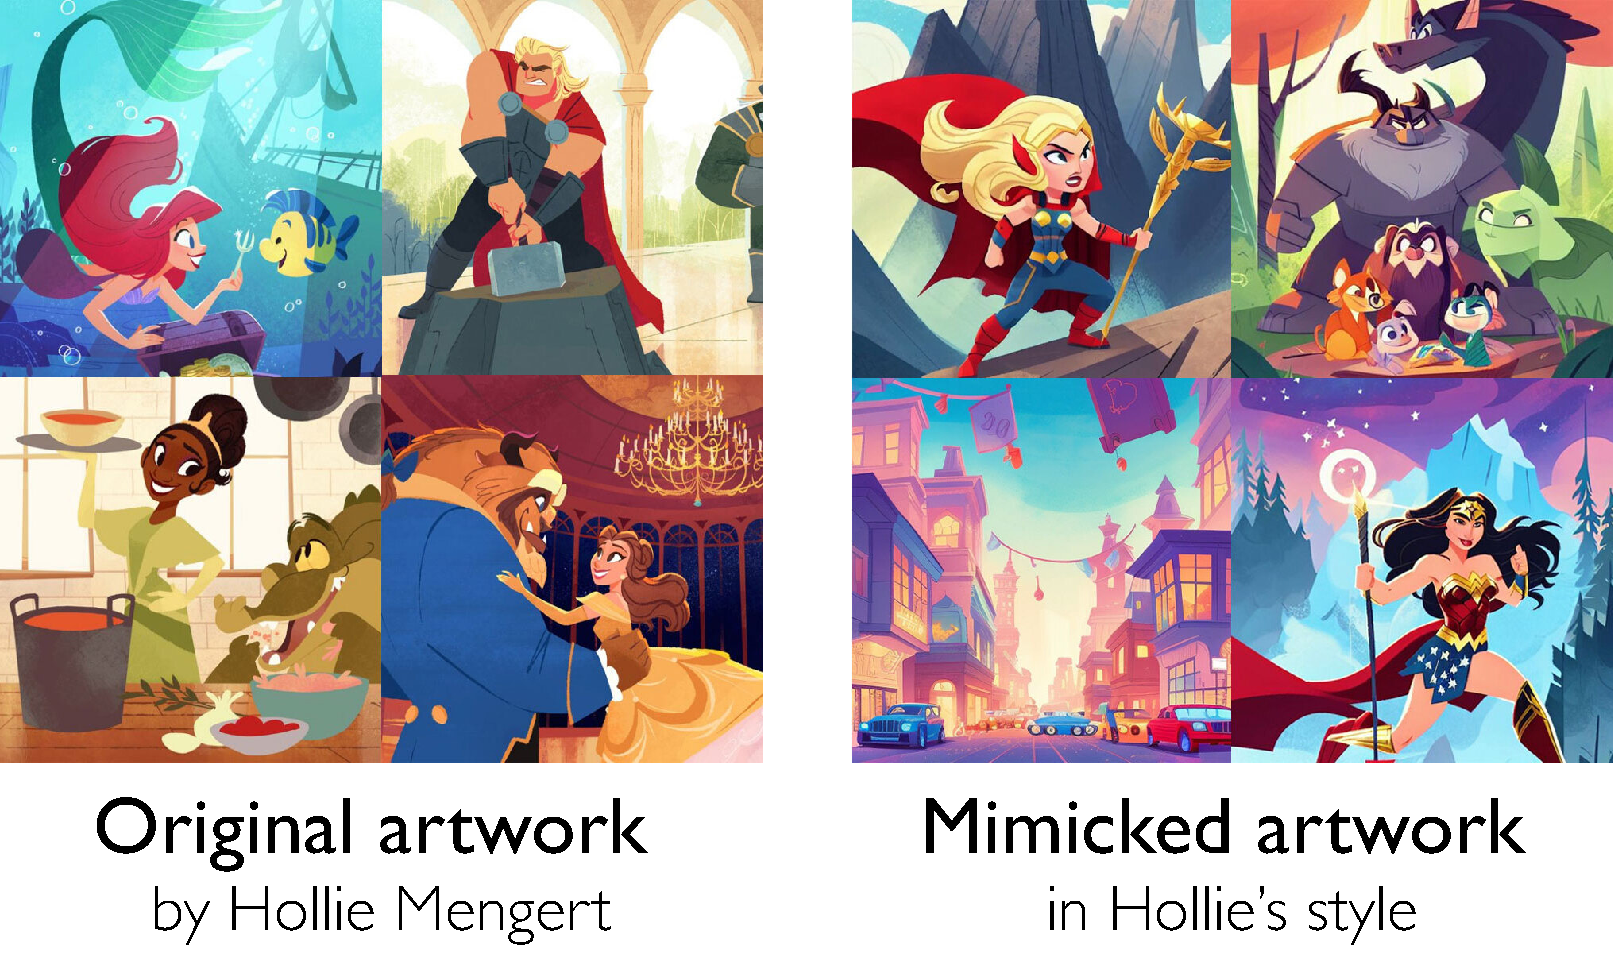
\includegraphics[width=0.95\columnwidth]{plots/overview/hollie-mimic.pdf}
  \vspace{-0.1in}
  \caption{Real-world incident of AI plagiarizing the style of artist Hollie Mengert~\cite{hollie-steal}. {\bf Left}: original artwork by Hollie Mengert. {\bf Right}: plagiarized artwork generated by a model trained to mimic Hollie's style. }
  \label{fig:hollie-mimic}
\end{figure}

In a {\em style mimicry} attack, a bad actor uses an AI art model to create
art in a particular artist's style without their consent. % Style mimicry can
More than 67\% of 
art pieces showcased on a popular AI-art-sharing website leverage style
mimicry~\cite{mid-top-artistname}.

\para{Style mimicry techniques.} Today, a ``mimic'' can easily copy the style of
a victim artist with only an open-source text-to-image model and a few
samples of artwork from the artist. A naive mimicry attack directly queries a
generic text-to-image model using the name of the victim artist. For example,
the prompt ``a painting in the style of Greg Rutkowski'' would cause the
model to generate images in the style of Polish artist Greg Rutkowski. This
is because many of Rutkowski's artworks appear in training datasets of these
generic models labeled with his name.

Naive mimicry can succeed when the artist is well-known and
has a significant amount of art online, but fail on other artists. In more recent
mimicry attacks, a mimic {\em fine-tunes} a
generic text-to-image model on samples of a target artist's work
(as few as $20$ unique pieces) downloaded from online sources. This calibrates the model to
the victim artist's style, identifying important features related to the
victim style and associating these regions in the feature space with the
victim artist's name~\cite{ruiz2022dreambooth,gal2022image}. This enables
style mimicry with impressive accuracy.  The entire fine-tuning process takes
less than 20 minutes on a low-end consumer GPU\footnote{It takes an average
  of 18.3 minutes on a GTX 1080 GPU}.

\para{Real-work mimicry incidents. }
The first well-known incident of mimicry was when a Reddit user stole
American artist Hollie Mengert's style and open-sourced the style-specific
model on Reddit~\cite{hollie-steal}. Figure~\ref{fig:hollie-mimic} has a
side-by-side comparison of Hollie's original artwork and plagiarized artwork
generated via style mimicry. Later, famous cartoonist Sarah Andersen reported
that AI art models can mimic her cartoon drawings~\cite{sarah-andersen}, and
other similar incidents abound~\cite{lensa-steal,sam-steal}.

Several companies~\cite{aigame} have even hosted style mimicry
as a service, allowing users to upload a few art pieces painted by victim
artists and producing new art in the victim styles. CivitAI~\cite{civitai}
built a large online marketplace where people share their customized stable
diffusion models, fine-tuned on certain artwork.  

\begin{figure}[t]
  \centering
  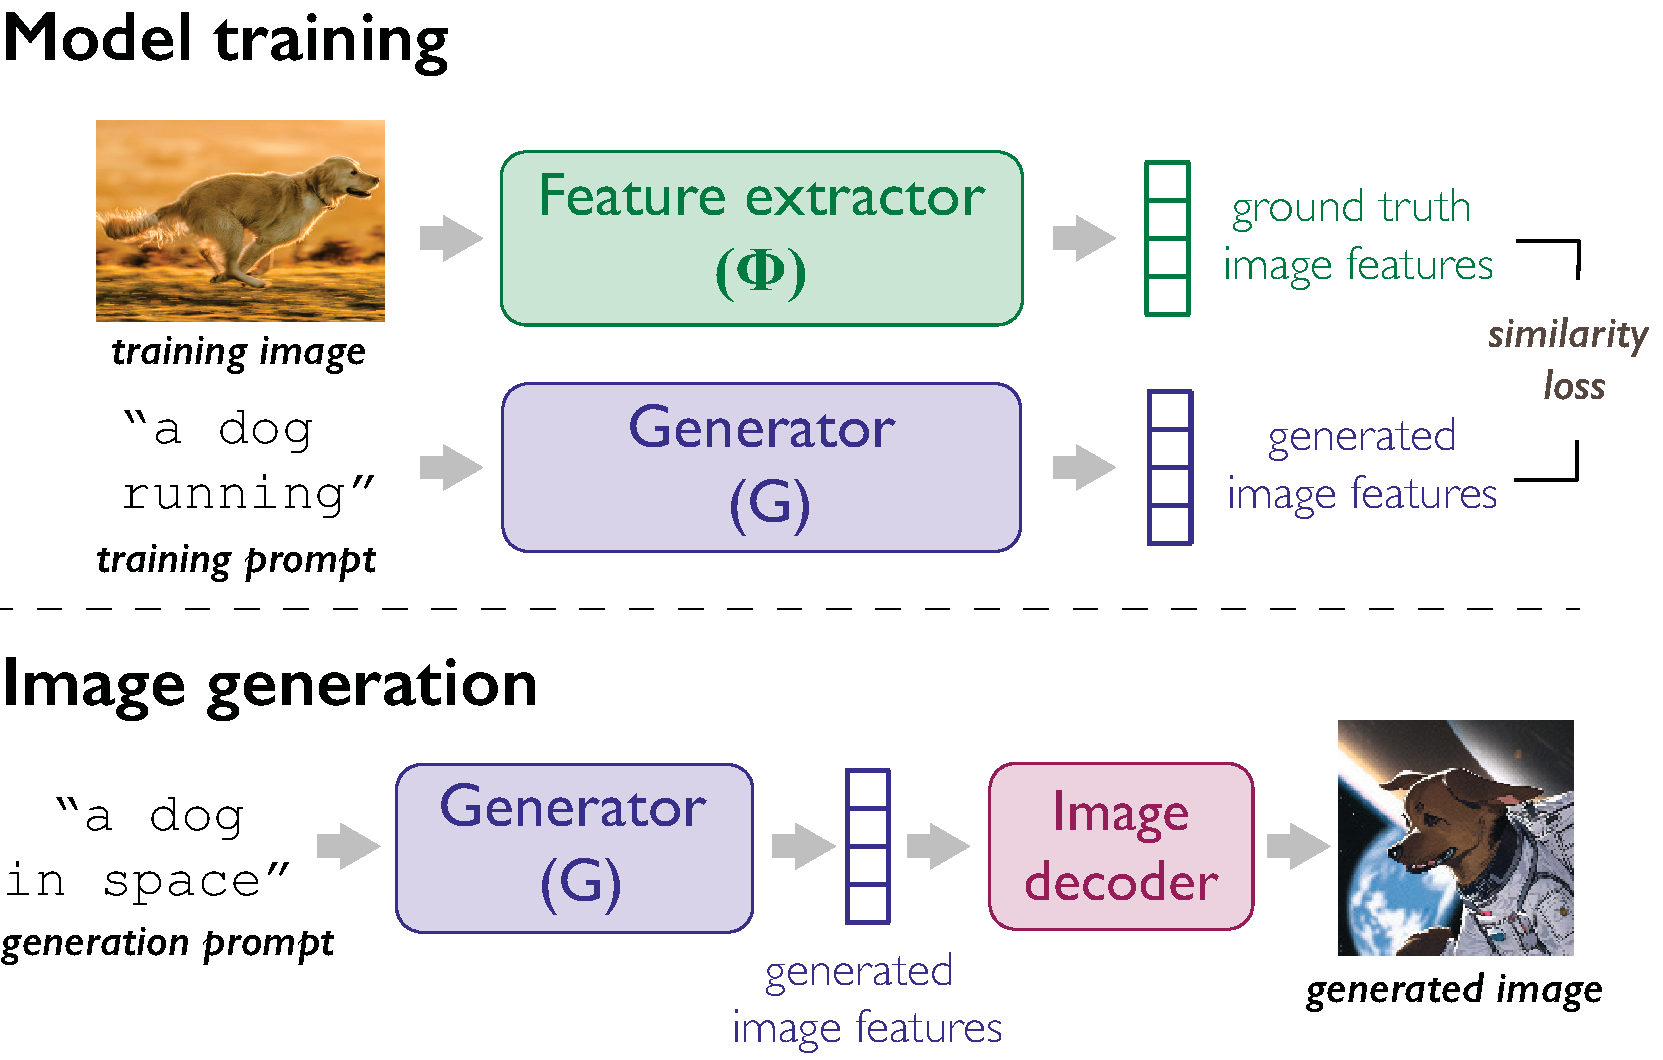
\includegraphics[width=1\columnwidth]{plots/overview/diffusion-arch.pdf}
  \vspace{-0.25in}
  \caption{High level model architecture of text-to-image models. }
  \label{fig:diffusion-arch}
\end{figure}

\secspace
\section{Collaborating with Artists}
\label{sec:artists}
Next, we explain our collaborative relationship with professional artists,
and its significant impact on our key evaluation metrics in this paper. We
also summarize key results from our first user study on views of AI art and
mimicry by members of the artist community.


Artists have spoken out against style mimicry in numerous venues, focusing
particularly on how it violates their intellectual property rights and
threatens their
livelihoods~\cite{guardian-artical,artical-1,artical-2, noai-protest}. Others
have taken direct action. The Concept Art Association raised over \$200K to
fight AI art, and filed a class action lawsuit in the US
against AI art companies~\cite{class-action}. In November 2022, artists
organized a large protest against ArtStation~\cite{noai-protest}, the large
digital art sharing platform that allowed users to post AI artwork without
identification. Anti-AI images flooded the site for several weeks, until
ArtStation banned the protest images~\cite{noai-result}. \revise{Recently, the
Writers Guild of America (WGA) went on strike demanding contractual changes
to ban generative AI~\cite{AIstrike}.}

Members of the professional art community reached out to us in Sept 2022. We
joined online town halls and meetings alongside hundreds of professionals,
including Emmy winners and artists at major film studios. After learning
more, we began an active collaboration with multiple professional artists,
including award-winning artist Karla Ortiz, who leads efforts defending
artists and is lead plaintiff in the class action suit.
The artists helped this project in multiple ways, by 1) sharing experiences
about specific ways AI-art has impacted them and their colleagues; 2) sharing
domain knowledge about what is acceptable to artists in terms of
perturbations on their art; and 3) helping to widely disseminate our user study to
members of their professional organizations, including the Concept Art
Association and the Animation Guild (TAG839).

\para{Evaluation via Direct Feedback from Artists.} Our goal is to help artists
disrupt AI models trying to mimic their artistic style, without adversely
impacting their own artwork. Because ``success'' in this context is highly
subjective (``Did this AI-art successfully mimic Karla's painting style?''),
we believe the only reliable evaluation metric is direct feedback by
professional artists themselves. Therefore, wherever possible, the evaluation
of \system{} is done via detailed user studies engaging members of the
professional artist community, augmented by an empirical score we develop based on
genre prediction using CLIP models.

We deployed two user studies during the course of this project (see
Table~\ref{tab:study-details}). Both are IRB-approved by our institution.  Both
draw participants from professional artists informed via their social circles
and professional networks. The first (Survey 1, \S\ref{sec:user-study},
\S\ref{sec:cloaking-results}), asked participants
about their broad views of AI style mimicry, and then presented them with a
number of inputs and outputs of our tool, and asked them to give ratings
corresponding to key metrics we wanted to evaluate. We select a subset 
of participants from the first study to participate in a 
longer and more in-depth study (Survey 2) where 
they were asked to evaluate the performance of \system{} in 
additional settings (\S\ref{sec:cloaking-results}, \S\ref{sec:robust-eval}, 
\S\ref{sec:counter}, and Appendix~\ref{sec:appendix}). 


\begin{table}[t]
  \centering
  \resizebox{0.49\textwidth}{!}{
  \centering
    \begin{tabular}{ccl}
    \hline
    \textbf{Survey} & \textbf{\begin{tabular}[c]{@{}c@{}} \# of artists\end{tabular}} & \multicolumn{1}{c}{\textbf{Content}} \\ \hline
    Survey 1 & 1156 & \begin{tabular}[c]{@{}l@{}} 1) Broad views of AI art
                        and style mimicry(\S\ref{sec:user-study}) \\
                        2) Glaze's usability, i.e. acceptable levels of cloaking (\S\ref{sec:cloaking-results}) \\
                        3) Glaze performance in disrupting style mimicry (\S\ref{sec:cloaking-results}) \end{tabular} \\ \hline
    
\begin{tabular}[c]{@{}c@{}}
    Survey 2\\(Extension to Survey 1)
    \end{tabular}
    & 151 & \begin{tabular}[c]{@{}l@{}}
    1) Additional performance tests (\S\ref{sec:cloaking-results}) \\
    2) Robustness to advanced scenarios (\S\ref{sec:robust-eval}) \\ and countermeasures (\S\ref{sec:counter}) \\ 
    3) Additional system evaluation (Appendix~\ref{sec:appendix}) \end{tabular} \\ \hline
    \end{tabular}
  }
  \vspace{-0.1in}
  \caption{Information on our user studies: the number of artist participants
    and where we report the results of the studies. We sent Survey 2 to
    some specific participants from survey 1 who volunteered to participate in a
    followup study.}
  \label{tab:study-details}
\end{table}


\secspace
\subsection{Artists' Opinions on Style Mimicry}
\label{sec:user-study}

While we expected artists to view style mimicry negatively, we wanted to
better understand how much individual artists understood this topic and how
many perceived it as a threat. Here we describe results from Survey 1 to
gather perceptions of the potential impact of AI art on existing artists.

\para{Survey Design.} Our survey consisted of both multiple choice and free
response questions to understand how well people understand the concept of AI
art, and how well the models successfully imitate the style of artists.
Additionally, we asked artists about the extent to which they anticipate the
emergence of AI art to impact their artistic activities, such as posting
their art online and their job security.  A handful of professional artists
helped disseminate our survey to their respective artist community groups.
Overall, we collected responses from 1,207 participants, consisting primarily
of professional artists (both full-time (46\%) and part-time/freelancer
(50\%)) and some non-artist members of the art community who felt invested in
the impact of AI art (4\%). Of the participants who consider themselves
artists, their experience varied: <1 year (13\%), 1-5 years (49\%), 5-10
years (19\%), 10+ years (19\%).  Participants' primary art style varied
widely, including: animation, concept art, abstract, anime, game art, digital
2D/3D, illustration, character artwork, storyboarding, traditional
painting/drawing, graphic design, and others.

\para{Key Results.} Our study found that 91\% of the artists have read about
AI art extensively, and either know of or worry about their art being used to
train the models. Artists expect AI mimicry to have a significant impact on artist
community: $97\%$ artists state it will decrease some artists' job security;
$88\%$ artists state it will discourage new students from studying art; and
$70\%$ artists state it will diminish creativity. ``Junior positions will
become extinct,'' as stated by one participant.

Many artists (> 89\% artists) have already or plan to take actions because of
AI mimicry. Over $95\%$ of artists post their artwork online. Out of these
artists, $53\%$ of them anticipate reducing or removing their online artwork,
if they haven't already. Out of these artists, $55\%$ of them believe
reducing their online presence will significantly impact their careers. One
participant stated ``AI art has unmotivated myself from uploading more art
and made me think about all the years I spent learning art.'' $78\%$ of
artists anticipate AI mimicry would impact their job security, and this
percentage increases to $94\%$ for the job security of newer
artists. Further, $24\%$ of artists believe AI art has \textit{already}
impacted their job security, and an additional $53\%$ expect to be affected
within the next 3 years. Over $51\%$ of artists expressed interest in
proactive measures, such as personally joining class action lawsuits against
AI companies.  

Professional artists thought AI mimicry was very successful at mimicking the
style of specific artists.  We showed the artists examples of original
artwork from $23$ artists, and the artwork generated by a model
attempting to mimic their styles (detailed mimicry setup in
\S\ref{sec:eval-cloak}).  $77\%$ of artists found the AI model
\textit{successfully} or \textit{very successfully} mimic the styles of
victim artists, with one stating ``it's shocking how well AI can mimic the
original artwork.''  Additionally, $19\%$ of participants thought the AI
mimicry is somewhat successful, leaving only $< 5\%$ of artists rating the
mimicry as unsuccessful.  Several artists also pointed out that, as artists,
upon close inspection they could spot differences between the AI art and
originals, but were skeptical the general public would notice them.
%the same disparities.

A significant concern of most participants, surprisingly, is not just the
existence of AI art, but rather scraping of existing artworks without
permission or compensation.  As one participant stated: ``If artists are paid
to have their pieces be used and asked permission, and if people had to pay
to use that AI software with those pieces in it, I would have no problem.''
However, without consent to use their artwork to train the models, ``it's
incredibly disrespectful to the artist to have their work `eaten' by a
machine [after] many years to grow our skills and develop our styles.''
%
\section{Background and Related Work}
\label{sec:back}

We begin by providing background on style mimicry and existing image-based protection methods. Then we follow with an overview of publicly available tools that enable style mimicry attacks on the video domain.

\subsection{Style Mimicry and Existing Defenses}
\label{sec:back1}
In a style mimicry attack, a bad actor finetunes a text-to-image model to
generate art in a particular artist's style without their consent. 
Since the introduction of text-to-image diffusion~\cite{sd-release,podell2023sdxl,df,novelai-update,ramesh2022hierarchical} models in 2022, style mimicry has grown significantly. There have been multiple high-profile mimicry incidents involving human artists~\cite{hollie-steal,sarah-andersen,lensa-steal,sam-steal}, and new companies are founded that focus purely on style mimicry~\cite{aigame,lexica}. AI marketplaces have also recently gained traction, with websites like CivitAI~\cite{civitai} offering over 119K ready-to-use mimicry models for people to download and use.

\para{Image-based style mimicry. } 
Style mimicry relies on finetuning pretrained text-to-image models (\eg stable diffusion) on a small set of images from a specific style~\cite{ruiz2022dreambooth,finetune-c,gal2022image}. The quality of these images greatly impacts the mimicry result, and thus, attackers often scrape high quality images from artists' websites and online galleries~\cite{hollie-steal,sam-steal}. In practice, a bad actor does not need many (less than 20 images~\cite{shan2023glaze,gal2022image}) in order to successfully generate arbitrary artwork from a victim artist's style. Because of the risk of image-based mimicry, many artists choose to reduce the amount of art they post online~\cite{aiprotest}, reduce the quality of any posted art~\cite{lowres}, and apply protection (discussed in details below) on this artwork~\cite{shan2023glaze}. 

\para{Protecting images from style mimicry. } 
Existing work (Mist~\cite{mist}, Anti-Dreambooth~\cite{antidb}, and Glaze \cite{shan2023glaze}) has 
proposed methods that leverage clean-label poisoning~\cite{saha2020hidden, turner2018clean, zhu2019transferable} to prevent style mimicry. At a high level, these systems add small optimized perturbations to image artwork that modifies the perturbed image's feature space representation without altering its content. The altered feature space representation prevents models from learning the correct artistic style. In general, these protection tools calculate the perturbation $\delta_x$ for an image $x$ using the following objective: 

\secspace
\begin{eqnarray}
   &\min\limits_{\delta_x} Dist\left( \Phi(x + \delta_x), \Phi(T)\right),  \label{eq:cloakopt}\\
  & \text{subject to } \; |\delta_x|< p, \nonumber
\end{eqnarray} 

where $\Phi$ is a generic image feature extractor from a public text-to-image model, $Dist(.)$ computes the distance between two feature representations, $|\delta_x|$ measures the perceptual perturbation caused by protection, and $p$ is the perceptual perturbation budget. $T$ is 
a ``target image'' that the perturbation $\delta_x$ is optimized towards, such that $x + 
\delta_x$ resembles $T$ in feature space while being visually identical to $x$. Mist~\cite{mist} extends the optimization objective across the entire diffusion process, including gradient computations through the randomized diffusion denoising process. By default, Mist uses a predefined black and white patterned image as its target with the goal of producing chaotic patterns in generated images. Anti-DB (Anti-Dreambooth)~\cite{antidb} is most similar to Mist, but modifies the optimization objective to specifically target Dreambooth~\cite{ruiz2022dreambooth} text-to-image models. There, they find that training surrogate models alongside computing image perturbations results in stronger protection, though it incurs additional computation time. Glaze~\cite{shan2023glaze} introduces input-specific target images by performing style transfer on the input image using a contrasting artistic style. This method preserves the overall content of the input image, while changing mainly the style, which the authors argue leads to more robust protection. Glaze then attacks the image encoder of a diffusion model as detailed above. 

These protection tools have been positively received by the artist community,
with Glaze having been downloaded at least 2.3 million
times~\cite{shan2023glazewebsite}. While these systems are typically too
computationally expensive for artists, efforts have been made to improve
accessibility~\cite{mistgithub, shan2023webglaze}. Since these systems are
free and increasingly available, images may no longer be a viable data source
for attackers to access artwork for fine-tuning text-to-image models. 

Video protection, on the other hand, has yet to be explored. Computation time per image is already limiting for many artists, and applying the same algorithms to all frames would be many times more costly. Yet, videos represent a significant source of data, incentivizing attackers to explore publicly available video art, such as short animation, movies or video game trailers etc..

Until recently, most style mimicry models are trained on still images. This 
is no longer the case today because 1) artists are increasingly more reluctant to post their 
work on the Internet~\cite{aiprotest}, 2) existing defenses (\S\ref{sec:back1}) are effective at protecting still images against mimicry, 3) video frames offer a significantly more diverse range of images compared to still images. 

\para{Video content is a promising source for mimicry. } 
Video content (\eg game trailers, anime, short videos, documentary, ads) provides promising alternative data sources for two reasons. First, video contents often offer a more diverse (3D) shots of an object or style, \eg rotating shot of an object, panning across a scene. These diverse viewpoints 
enable models to better learn the content during the training process~\cite{videomotivate}. Second, there are significantly more video frames compared to still images and many of the videos contain unique art styles/characters. The entire Internet produces around 3.2 billions still images daily~\cite{manyvideos}, while YouTube alone sees over 271,000 hours of videos (\ie around 29 billions video frames) uploaded per day. Specifically, gaming companies and animation studios often use short videos as a way to promote new games, characters, and movies. Movie clip compilations and trailers are readily available on YouTube~\cite{movietrailers}, while video game companies like Riot and Mihoyo frequently post teasers and trailers showcasing new playable content, or highly anticipated characters~\cite{genshintrailer, leaguetrailer}. These videos are filled with original artwork, and contain image frames that are prime targets for style mimicry. 

\para{Video-based mimicry in the real-world. } 
Style mimicry using video content has already occurred in the real-world. Bad actors have created and distributed software that generates high quality text-to-image datasets from online videos. One GitHub tool~\cite{anime2sd} automates the process of downloading (\eg torrenting) Japanese Anime episodes and extracting high quality frames of desired characters. Another option~\cite{civitai-video} advertised on CivitAI does the same, with the additional capability of scraping frames from screencap websites such as FanCaps~\cite{fancaps}. These tools demonstrate that there already exists sophisticated technology aimed at creating text-to-image datasets from original video content. 

We also provide our own examples of this threat. We download and extract high quality frames from YouTube videos and train style mimicry models on them (Figure~\ref{fig:style-mimicry-scenario}). Figure~\ref{fig:style-mimicry-baseline} shows some examples of extracted video frames as well as mimicry results generated by the style mimicry model. We include human evaluation of the success of these style mimicry images later using user studies with both artists and the general public in \S\ref{sec:eval}. 

While there has been recent developments in text-to-video~\cite{videoworldsimulators2024} and image-to-video models~\cite{blattmann2023stable}, we leave them as a topic for future work, and focus solely on text-to-image mimicry where the source of data originates from video content. 


\section{Methodology}
\ours follows the same framework as speculative decoding, where each decoding step primarily consists of three substeps: (1) generating candidates, (2) processing candidates, and (3) accepting candidates. For \ours, (1) is achieved by \ours heads, (2) is realized by tree attention, and since \ours heads are on top of the original model, the logits calculated in (2) can be used for substep (1) for the next decoding step. The final step (3) can be realized by either rejection sampling~\citep{leviathan2022fast,chen2023accelerating} or typical acceptance (Section~\ref{sec:typical_acceptance}). The overall pipeline is illustrated in Figure~\ref{fig:pipeline}.

In this section, we first introduce the key components of \ours, including \ours heads, and tree attention. Then, we present two levels of fine-tuning procedures for \ours to meet the needs of different use cases. Finally, we propose two extensions to \ours, including self-distillation and typical acceptance, to handle situations where no training data is available for \ours and to improve the efficiency of the decoding process, respectively.
\subsection{Key Components}
\subsubsection{\ours Heads}
\label{sec:medusa_heads}
In speculative decoding, subsequent tokens are predicted by an auxiliary draft model. This draft model must be small yet effective enough to generate continuations that the original model will accept. Fulfilling these requirements is a challenging task, and existing approaches~\citep{spector2023accelerating,miao2023specinfer} often resort to separately \emph{pre-training} a smaller model. This pre-training process demands substantial additional computational resources. For example, in \citep{miao2023specinfer}, a reported 275 NVIDIA A100 GPU hours were used. Additionally, separate pre-training can potentially create a distribution shift between the draft model and the original model, leading to continuations that the original model may not favor. \citet{chen2023accelerating} have also highlighted the complexities of serving multiple models in a distributed environment.

\textcolor{black}{To streamline and democratize the acceleration of LLM inference, we take inspiration from \citet{stern2018blockwise}, which utilizes parallel decoding for tasks such as machine translation and image super-resolution. \ours heads}
 are additional decoding heads appended to the last hidden states of the original model. Specifically, given the original model's last hidden states $h_t$ at position $t$, we add $K$ decoding heads to $h_t$. The $k$-th head is used to predict the token in the $(t+k+1)$-th position of the next tokens (the original language model head is used to predict the $(t+1)$-th position). The prediction of the $k$-th head is denoted as $p_t^{(k)}$, representing a distribution over the vocabulary, while the prediction of the original model is denoted as $p_t^{(0)}$. Following the approach of \citet{stern2018blockwise}, we utilize a single layer of feed-forward network with a residual connection for each head. We find that this simple design is sufficient to achieve satisfactory performance. The definition of the $k$-th head is outlined as:

\begin{align*}
p_t^{(k)} = \text{softmax}\left(W_2^{(k)} \cdot \left(\text{SiLU}(W_1^{(k)} \cdot h_t)+h_t\right)\right),\\
\text{where } W_2^{(k)}\in\mathbb{R}^{d\times V}, W_1^{(k)}\in\mathbb{R}^{d\times d}.
\end{align*}

\textcolor{black}{$d$ is the output dimension of the LLM's last hidden layer and $V$ is the vocabulary size.}
\textcolor{black}{We initialize $W_2^{(k)}$ identically to the original language model head, and $W_1^{(k)}$ to zero.}
This aligns the initial prediction of \ours heads with that of the original model. The SiLU activation function~\citep{elfwing2017sigmoidweighted} is employed following the Llama models~\citep{touvron2023llama}.

Unlike a draft model, \ours heads are trained in conjunction with the original backbone model, which can remain \emph{frozen} during training (\ours-1) or be trained together (\ours-2). This method allows for fine-tuning large models even on a single GPU, taking advantage of the powerful base model's learned representations. Furthermore, it ensures that the distribution of the \ours heads aligns with that of the original model, thereby mitigating the distribution shift problem. Additionally, since the new heads consist of just a single layer akin to the original language model head, \ours does not add complexity to the serving system design and is friendly to distributed settings. We will discuss the training recipe for \ours heads in Section~\ref{sec:training_recipe}.

\subsubsection{Tree Attention}
\label{sec:tree_attention}
Through \ours heads, we obtain probability predictions for the subsequent $K+1$ tokens. These predictions enable us to create length-$K+1$ continuations as candidates. While the speculative decoding studies~\citep{leviathan2022fast,chen2023accelerating} suggest sampling a single continuation as the candidate, leveraging multiple candidates during decoding can enhance the expected acceptance length within a decoding step. Nevertheless, more candidates can also raise computational demands. To strike a balance, we employ a tree-structured attention mechanism to process multiple candidates concurrently.
\begin{figure}[ht]
    \centering
    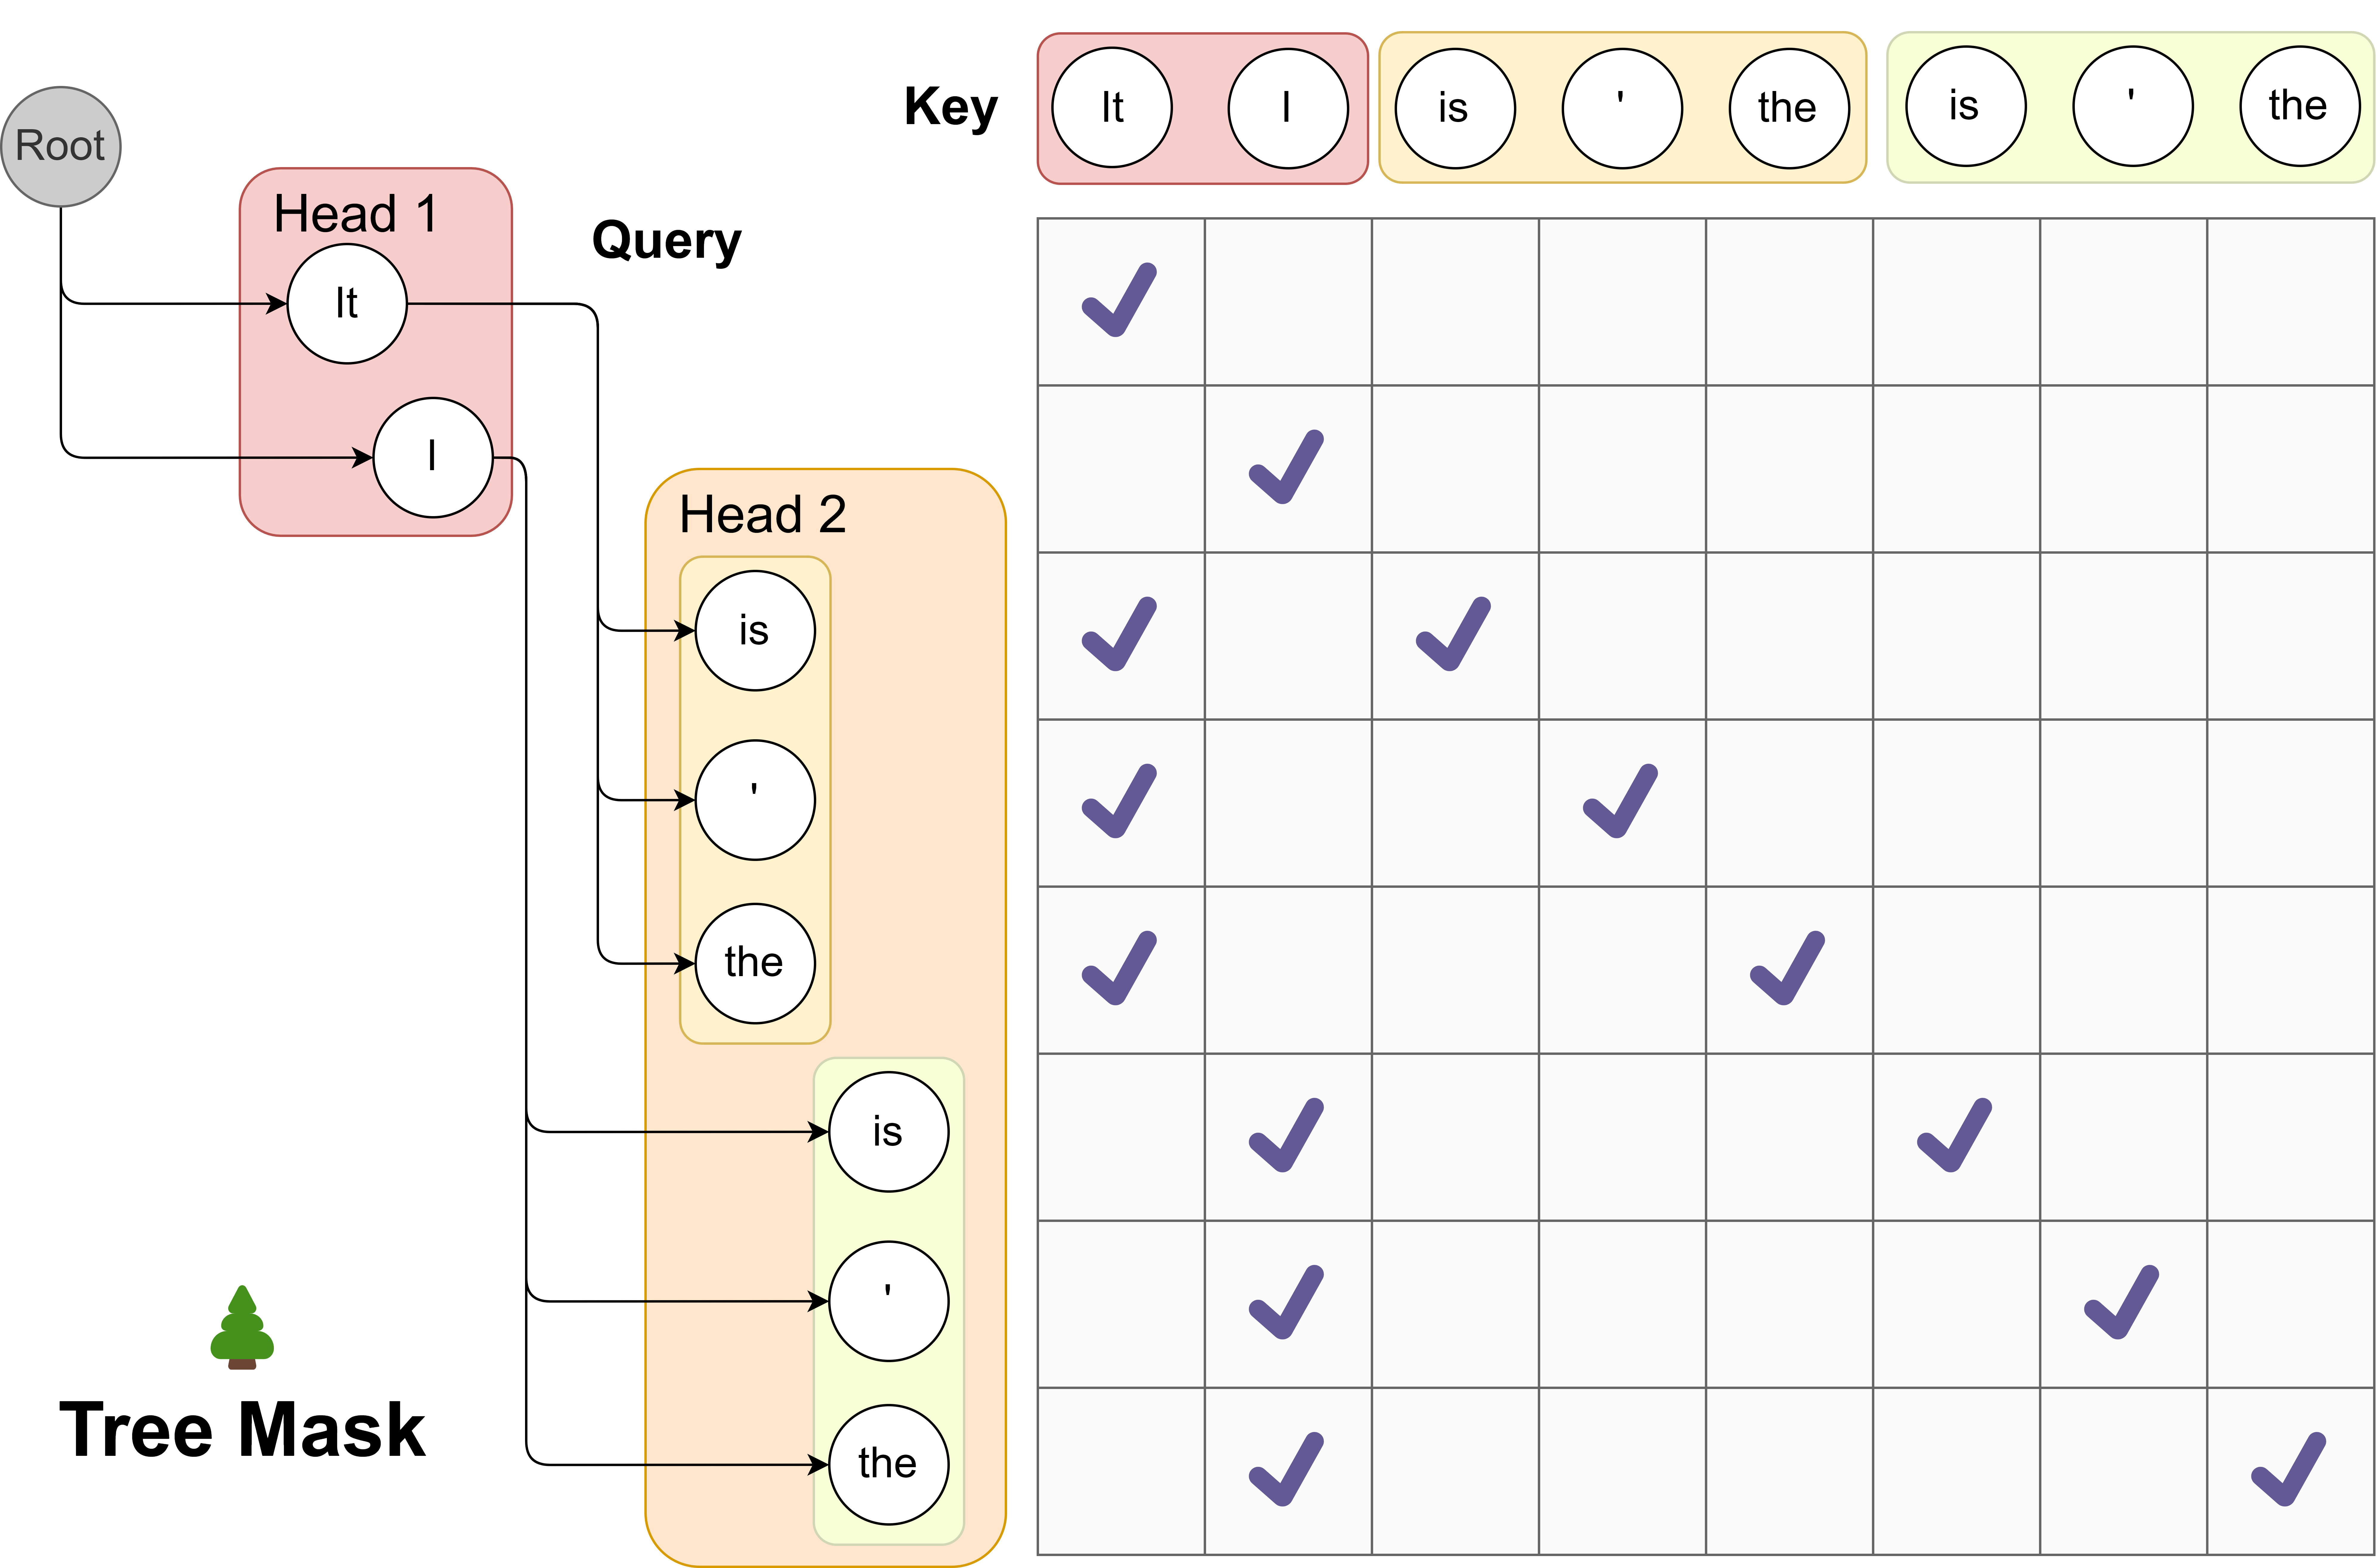
\includegraphics[width=0.45\textwidth]{tree_attention.png}
    \caption{
    We demonstrates the use of tree attention to process multiple candidates concurrently. As exemplified, the top-2 predictions from the first \ours head and the top-3 from the second result in a total of $2\times3=6$ candidates. Each of these candidates corresponds to a distinct branch within the tree structure. To guarantee that each token only accesses its predecessors, we devise an attention mask that exclusively permits attention flow from the current token back to its antecedent tokens. The positional indices for positional encoding are adjusted in line with this structure.}
    \label{fig:tree_attention}
\end{figure}
This attention mechanism diverges from the traditional causal attention paradigm. Within this framework, only tokens from the same continuation are regarded as historical data. Drawing inspiration from the concept of embedding graph structures into attention as proposed in the graph neural network domain~\citep{ying2021transformers}, we incorporate the tree structure into our attention mask, visualized in Figure~\ref{fig:tree_attention}. Remarkably, similar ideas have also been explored in independent works like \citet{miao2023specinfer,spector2023accelerating}, where they follow a bottom-up approach and construct the tree by merging multiple candidates generated by a draft model. In our method, we instead take a top-down approach to build the tree thanks to the structure of candidates generated by \ours heads. For a given $k$-th head, its top-$s_k$ predictions serve as the basis for candidate formation, where $s_k$ is a designated hyperparameter. These candidates are established by determining the Cartesian product of the top-$s_k$ predictions from each head. For instance, in Figure~\ref{fig:tree_attention}, with $s_1=2$ and $s_2=3$, each first head prediction can be succeeded by any prediction from the second head. This leads to a tree structure where $s_k$ branches exist at the $k$-th level (considering a virtual root as the $0$-level, in practice, this $0$-level is for the prediction of the language model head of the original model, which can be sampled independently). Within this tree, only a token's predecessors are seen as historical context, and our attention mask ensures that the attention is only applied on a token's predecessors. By employing this mask and properly setting the positional indices for positional encoding, we can process numerous candidates simultaneously without the need to expand the batch size. The cumulative number of new tokens is calculated as $\sum_{k=1}^K \prod_{i=1}^k s_i$.

In this section, we demonstrate the most simple and regular way to construct the tree structure by taking the Cartesian product. However, it is possible to construct the tree structure in a more sophisticated way and exploit the unbalanced accuracy of different top predictions of different heads. We will discuss this in Section~\ref{sec:optimized_tree_construction}.
\subsection{Training Strategies}
\label{sec:training_recipe}
At the most basic level, we can train \ours heads by freezing the backbone model and fine-tuning \ours heads. However, training the backbone in conjunction with the \ours heads can significantly enhance the accuracy of the \ours heads. Depending on the computational resources and the specific reqirements of the use case, we propose two levels of training strategies for \ours heads.

In this section, we assume the availability of a training dataset that aligns with the target model’s output distribution. This could be the dataset used for Supervised Fine-Tuning (SFT) of the target model. We will discuss eliminating the need for such a dataset using a self-distillation approach in Section~\ref{sec:self_distillation}.
\subsubsection{\ours-1: Frozen Backbone}
\label{sec:frozen_backbone}
To train \ours heads with a frozen backbone model, we can use the cross-entropy loss between the prediction of \ours heads and the ground truth. Specifically, given the ground truth token $y_{t+k+1}$ at position $t+k+1$, the loss for the $k$-th head is $\mathcal{L}_k = -\log p_t^{(k)}(y_{t+k+1})$ where $p_t^{(k)}(y)$ denotes the probability of token $y$ predicted by the $k$-th head. We also observe that $\mathcal{L}_k$ is larger when $k$ is larger, which is reasonable since the prediction of the $k$-th head is more uncertain when $k$ is larger. Therefore, we can add a weight $\lambda_k$ to $\mathcal{L}_k$ to balance the loss of different heads. And the total \ours loss is:
\begin{align}
    \label{eq:loss_medusa_1}
    \mathcal{L}_{\text{\ours-1}} = \sum_{k=1}^K -\lambda_k\log p_t^{(k)}(y_{t+k+1}).
\end{align}

In practice, we set $\lambda_k$ as the $k$-th power of a constant like $0.8$. Since we only use the backbone model for providing the hidden states, we can use a quantized version of the backbone model to reduce the memory consumption. This introduces a more democratized way to accelerate LLM inference, as with the quantization, \ours can be trained for a large model on a single consumer GPU similar to QLoRA~\citep{dettmers2023qlora}. The training only takes a few hours (e.g., 5 hours for \ours-1 on Vicuna 7B model with a single NVIDIA A100 PCIE GPU to train on 60k ShareGPT samples).
\subsubsection{\ours-2: Joint Training}
\label{sec:joint_training}
To further improve the accuracy of \ours heads, we can train \ours heads together with the backbone model. However, this requires a special training recipe to preserve the backbone model's next-token prediction capability and output quality. To achieve this, we propose three strategies:
\begin{itemize}
    \item \textbf{Combined loss}: To keep the backbone model's next-token prediction capability, we need to add the cross-entropy loss of the backbone model $\mathcal{L}_{\text{LM}}=-\log p_t^{(0)}(y_{t+1})$ to the \ours loss. We also add a weight $\lambda_0$ to balance the loss of the backbone model and the \ours heads. Therefore, the total loss is:
    \begin{align}
        \label{eq:loss_medusa_2}
        \mathcal{L}_{\text{\ours-2}} = \mathcal{L}_{\text{LM}} + \lambda_0\mathcal{L}_{\text{\ours-1}}.
    \end{align}
    \item \textbf{Differential learning rates}: Since the backbone model is already well-trained and the \ours heads need more training, we can use separate learning rates for them to enable faster convergence of \ours heads while preserving the backbone model's capability.
    \item \textbf{Heads warmup}: Noticing that at the beginning of training, the \ours heads have a large loss, which leads to a large gradient and may distort the backbone model's parameters. Following the idea from \citet{kumar2022finetuning}, we can employ a two-stage training process. In the first stage, we only train the \ours heads as \ours-1. In the second stage, we train the backbone model and \ours heads together with a warmup strategy. Specifically, we first train the backbone model for a few epochs, then train the \ours heads together with the backbone model. Besides this simple strategy, we can also use a more sophisticated warmup strategy by gradually increasing the weight $\lambda_0$ of the backbone model's loss. We find both strategies work well in practice.
\end{itemize}
Putting these strategies together, we can train \ours heads together with the backbone model without hurting the backbone model's capability. Moreover, this recipe can be applied together with Supervised Fine-Tuning (SFT), enabling us to get a model with native \ours support.
\subsubsection{How to Select the Number of Heads}
Empirically, we found that five heads are sufficient at most. Therefore, we recommend training with five heads and referring to the strategy described in Section~\ref{sec:optimized_tree_construction} to determine the optimal configuration of the tree attention. With optimized tree attention, sometimes three or four heads may be enough for inference. In this case, we can ignore the redundant heads without overhead.

\subsection{Extensions}
\subsubsection{Typical Acceptance}
\label{sec:typical_acceptance}
In speculative decoding papers~\citep{leviathan2022fast,chen2023accelerating}, authors employ rejection sampling to yield diverse outputs that align with the distribution of the original model. However, subsequent implementations~\citep{gante2023assisted,spector2023accelerating} reveal that this sampling strategy results in diminished efficiency as the sampling temperature increases. Intuitively, this can be comprehended in the extreme instance where the draft model is the same as the original one\textcolor{black}{:} 
Using greedy decoding, all output of the draft model will be accepted, therefore maximizing the efficiency. 
Conversely, rejection sampling introduces extra overhead, as the draft model and the original model are sampled independently. Even if their distributions align perfectly, the output of the draft model may still be rejected.

However, in real-world scenarios, sampling from language models is often employed to generate diverse responses, and the temperature parameter is used merely to modulate the ``creativity'' of the response. Therefore, higher temperatures should result in more opportunities for the original model to accept the draft model's output. We ascertain that it is typically unnecessary to match the distribution of the original model. Thus, we propose employing a \emph{typical acceptance} scheme to select plausible candidates rather than using rejection sampling. This approach draws inspiration from truncation sampling studies~\citep{hewitt2022truncation} (refer to \textcolor{black}{Appendix}~\ref{sec:related_work} for an in-depth explanation). Our objective is to choose candidates that are \emph{typical}, meaning they are not exceedingly improbable to be produced by the original model. We use the prediction probability from the \emph{original model} as a natural gauge for this and establish a threshold based on the prediction distribution to determine acceptance. Specifically, given $x_1, x_2, \cdots, x_n$ as context, when evaluating the candidate sequence \textcolor{black}{$(x_{n+1}, x_{n+2}, \cdots, x_{n+K+1})$ }(composed by top predictions of the original language model head and \ours heads), we consider the condition
\begin{align*}
p_{\text{original}}(x_{n+k}|x_1, x_2, \cdots, x_{n+k-1}) > \\\min\rbr{\epsilon, \delta\exp\rbr{-H(p_{\text{original}}(\cdot|x_1, x_2, \cdots, x_{n+k-1}))}},
\end{align*}
where $H(\cdot)$ denotes the entropy function, and $\epsilon, \delta$ are \textcolor{black}{the hard threshold and the entropy-dependent
threshold respectively}. This criterion is adapted from \citet{hewitt2022truncation} and rests on two observations: (1) tokens with relatively high probability are meaningful, and (2) when the distribution's entropy is high, various continuations may be deemed reasonable. During decoding, every candidate is evaluated using this criterion, and a \emph{prefix} of the candidate is accepted if it satisfies the condition. To guarantee the generation of at least one token at each step, we apply \emph{greedy decoding} for the first token and \emph{unconditionally} accept it while employing typical acceptance for subsequent tokens. The final prediction for the current step is determined by the \emph{longest accepted prefix} among all candidates.

Examining this scheme leads to several insights. Firstly, when the temperature is set to $0$, it reverts to greedy decoding, as only the most probable token possesses non-zero probability. As the temperature surpasses $0$, the outcome of greedy decoding will consistently be accepted with appropriate $\epsilon, \delta$, since those tokens have the maximum probability, yielding maximal speedup. Likewise, in general scenarios, an increased temperature will correspondingly result in longer accepted sequences, as corroborated by our experimental findings.

Empirically, we verify that typical acceptance can achieve a better speedup while maintaining a similar \textcolor{black}{generation quality} as shown in Figure~\ref{fig:threshold_ablation}.
\subsubsection{Self-Distillation}
\label{sec:self_distillation}
In Section~\ref{sec:training_recipe}, we assume the existence of a training dataset that matches the target model's output distribution. However, this is not always the case. For example, the model owners may only release the model without the training data, or the model may have gone through a Reinforcement Learning with Human Feedback (RLHF) procedure, which makes the output distribution of the model different from the training dataset. To tackle this issue, we propose an automated self-distillation pipeline to use the model itself to generate the training dataset for \ours heads, which matches the output distribution of the model.

The dataset generation process is straightforward. We first take a public seed dataset from a domain similar to the target model; for example, using the ShareGPT~\citep{sharegpt2023} dataset for chat models. Then, we simply take the prompts from the dataset and ask the model to reply to the prompts. In order to obtain multi-turn conversation samples, we can sequentially feed the prompts from the seed dataset to the model. Or, for models like Zephyr 7B~\citep{tunstall2023zephyr}, which are trained on both roles of the conversation, they have the ability to self-talk, and we can simply feed the first prompt and let the model generate multiple rounds of conversation.

For \ours-1, this dataset is sufficient for training \ours heads. However, for \ours-2, we observe that solely using this dataset for training the backbone and \ours heads usually leads to a lower generation quality. In fact, even without training \ours heads, training the backbone model with this dataset will lead to performance degradation. This suggests that we also need to use the original model's probability prediction instead of using the ground truth token as the label for the backbone model, similar to classic knowledge distillation works~\citep{kim2016sequencelevel}. Concretely, the loss for the backbone model is:
\begin{align*}
    \mathcal{L}_{\text{LM-distill}} = KL(p_{\text{original},t}^{(0)}||p_t^{(0)}),
\end{align*}
where $p_{\text{original},t}^{(0)}$ denotes the probability distribution of the original model's prediction at position $t$.

However, naively, to obtain the original model's probability prediction, we need to maintain two models during training, increasing the memory requirements. To further alleviate this issue, we propose a simple yet effective way to exploit the self-distillation setup. We can use a parameter-efficient adapter like LoRA~\citep{hu2021lora} for fine-tuning the backbone model. In this way, the original model is simply the model with the adapter turned off. Therefore, the distillation does not require additional memory consumption. Together, this self-distillation pipeline can be used to train \ours-2 without hurting the backbone model's capability and introduce almost no additional memory consumption. Lastly, one tip about using self-distillation is that it is preferable to use LoRA without quantization in this case, otherwise, the teacher model will be the quantized model, which may lead to a lower generation quality.

\subsubsection{Searching for the Optimized Tree Construction}
\label{sec:optimized_tree_construction}
In Section~\ref{sec:tree_attention}, we present the simplest way to construct the tree structure by taking the Cartesian product. However, with a fixed budget for the number of total nodes in the tree, a regular tree structure may not be the best choice. Intuitively, those candidates composed of the top predictions of different heads may have different accuracies. Therefore, we can leverage an estimation of the accuracy to construct the tree structure.

Specifically, we can use a calibration dataset and calculate the accuracies of the top predictions of different heads. Let $a_k^{(i)}$ denote the accuracy of the $i$-th top prediction of the $k$-th head\footnote{Here, the accuracy is defined for the single top $i$-th token, i.e., this accuracy is equal to top-$i$ accuracy minus top-$(i-1)$ accuracy.}. Assuming the accuracies are independent, we can estimate the accuracy of a candidate sequence composed by the top $\sbr{i_1, i_2, \cdots, i_k}$ predictions of different heads as $\prod_{j=1}^k a_j^{(i_j)}$. Let $I$ denote the set of all possible combinations of $\sbr{i_1, i_2, \cdots, i_k}$ and each element of $I$ can be mapped to a node of the tree (not only leaf nodes but all nodes are included). Then, the expectation of the acceptance length of a candidate sequence is:
\begin{align*}
    \sum_{\sbr{i_1, i_2, \cdots, i_k}\in I}\prod_{j=1}^k a_j^{(i_j)}.
\end{align*}
Thinking about building a tree by adding nodes one by one, the contribution of a new node to the expectation is exactly the accuracy associated with the node. Therefore, we can greedily add nodes to the tree by choosing the node that is connected to the current tree and has the highest accuracy. This process can be repeated until the total number of nodes reaches the desired number. In this way, we can construct a tree that maximizes the expectation of the acceptance length. Further details can be found in Appendix~\ref{appendix:sparse_tree}.


\begin{figure}[t]
  \centering
  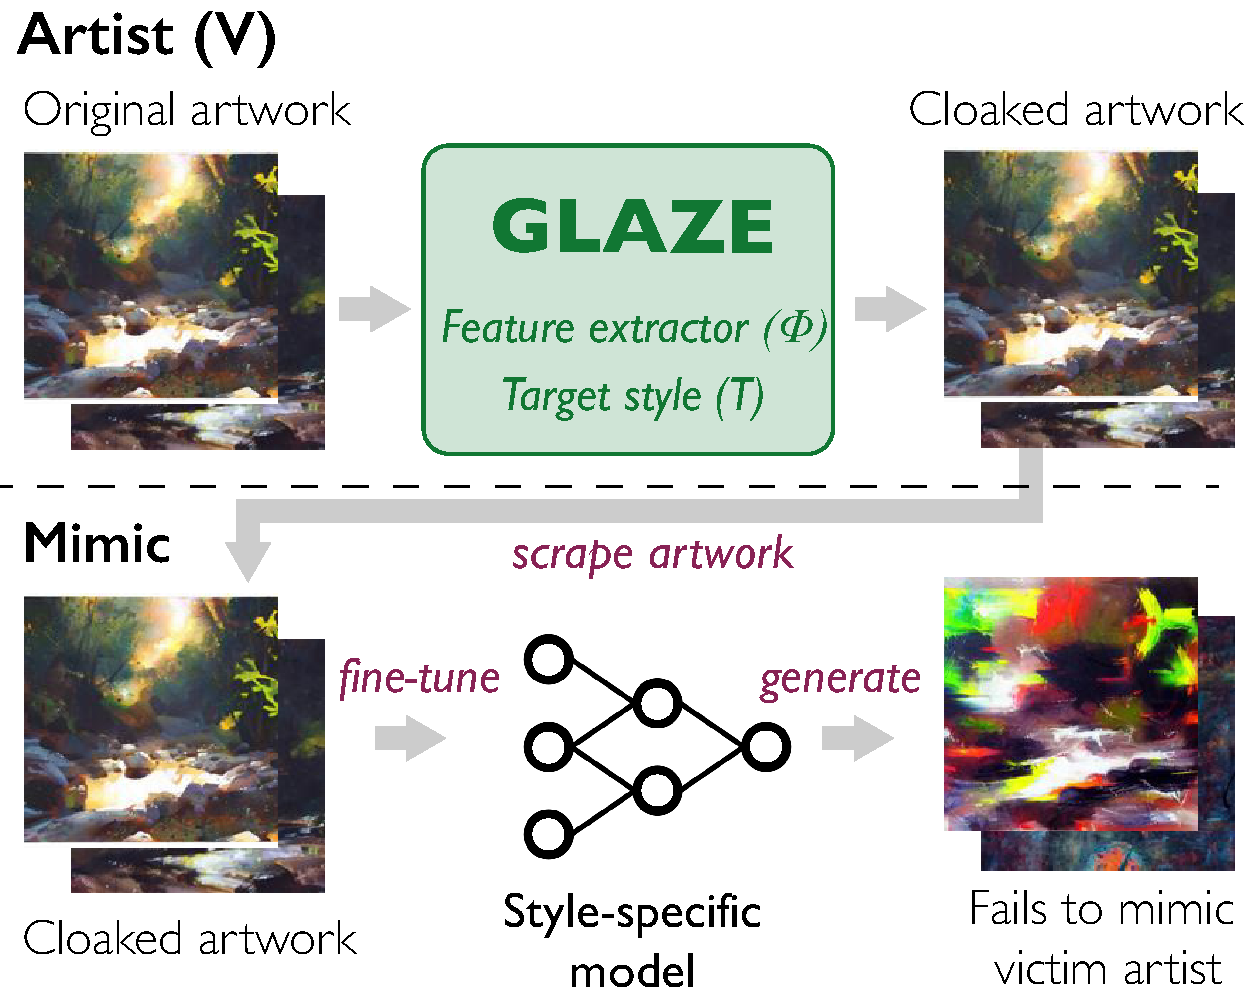
\includegraphics[width=0.9\columnwidth]{plots/overview/cloak-scenario-emily.pdf}
  \caption{Overview of \system{}, a system that protects victim artists from AI style mimicry by cloaking their online artwork. ({\bf Top}) An artist $V$ applies the cloaking algorithm (uses a feature extractor $\Phi$ and a target style $T$) to generate cloaked versions of $V$'s art pieces. Each cloak is a small perturbation unnoticeable to human eye. ({\bf Bottom}) A mimic scrapes the cloaked art pieces from online and uses them to fine-tune a model to mimic $V$'s style. When prompted to generate artwork in the style of $V$, mimic's model will generate artwork in the target style $T$, rather than $V$'s true style. }
  \label{fig:cloaking}
\end{figure}

\begin{figure}[t]
  \centering
  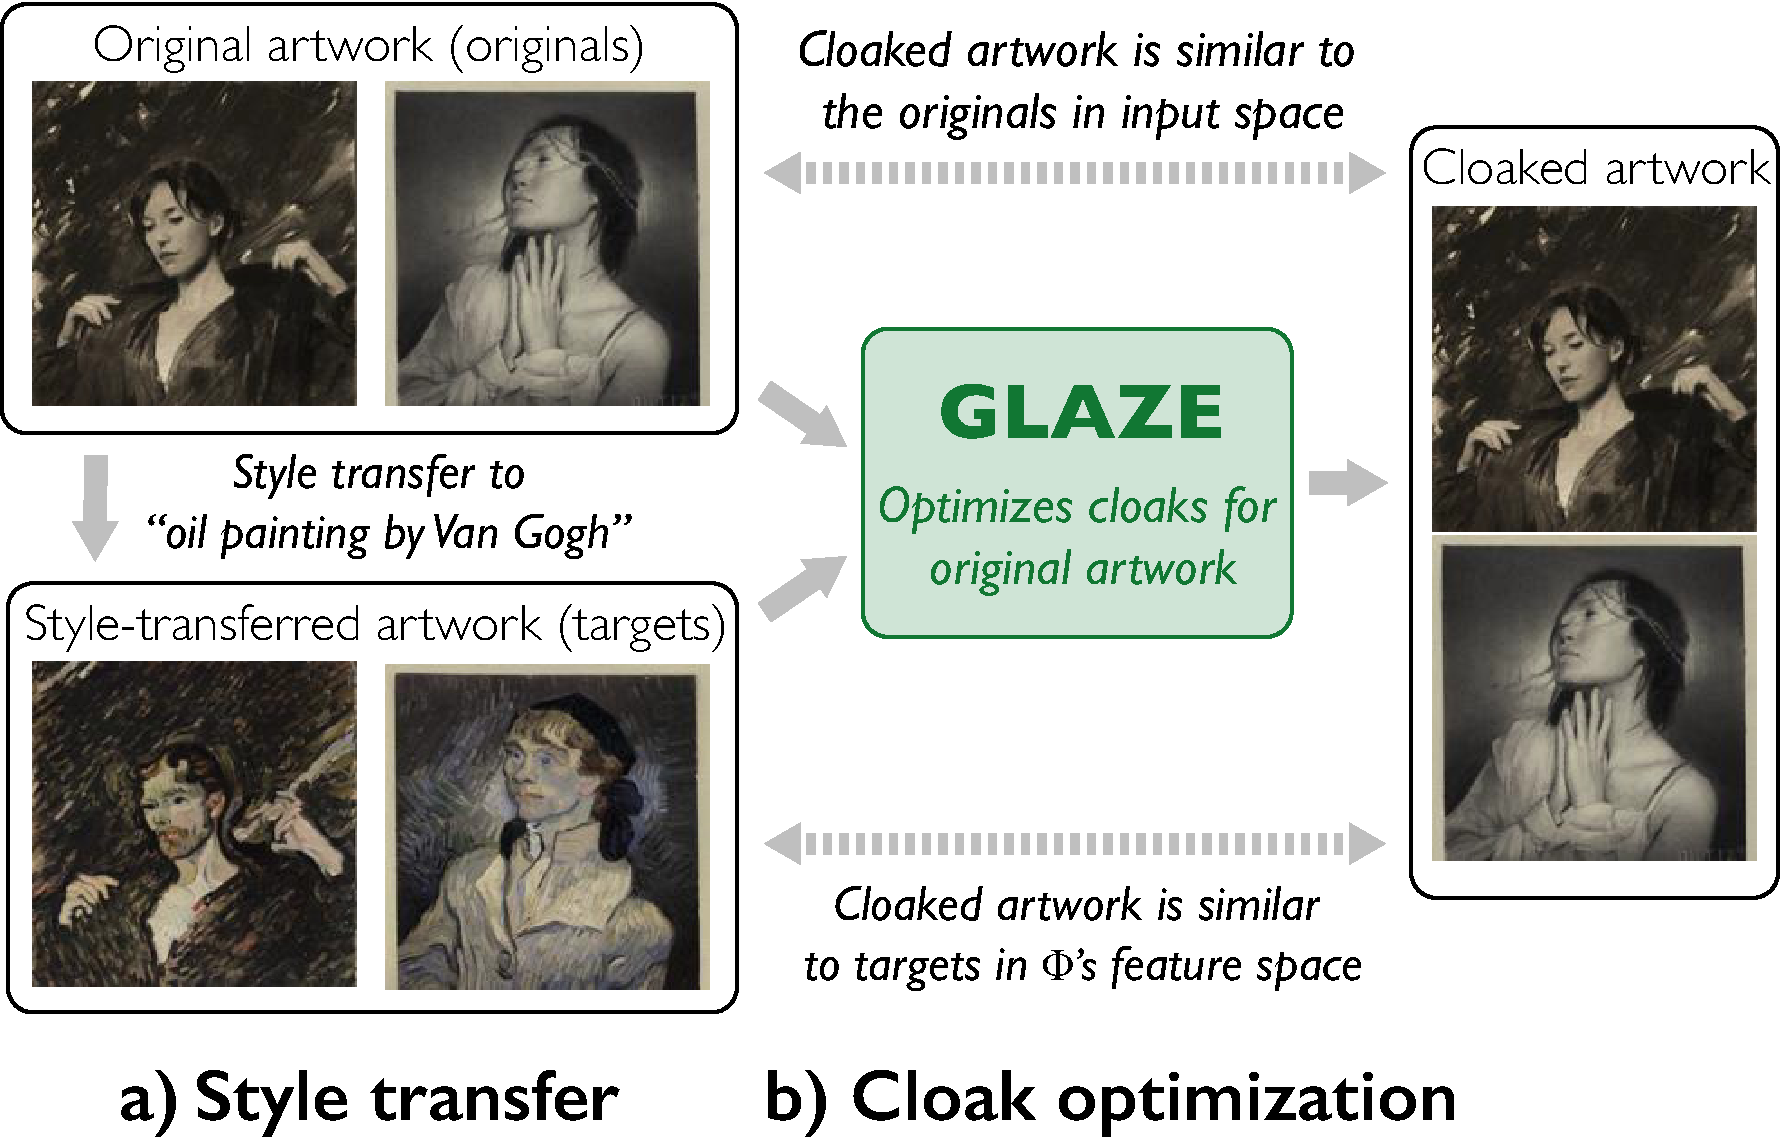
\includegraphics[width=1\columnwidth]{plots/overview/cloak-intuition-2-emily.pdf}
  \caption{High level overview of how \system{} perturbs the style-specific features of the artwork. {\bf a)} \system{} style transfers the original artwork to a different style, which changes its style but leaves other features unaltered. {\bf b)} \system{} optimizes a cloak that makes the artwork's features representation match that of the style-transferred art, while constraining the amount of visible changes to the artwork.  }
  \label{fig:cloak-intuition}
  \vspace{-0.3cm}
\end{figure}

\begin{figure}[t]
  \centering
  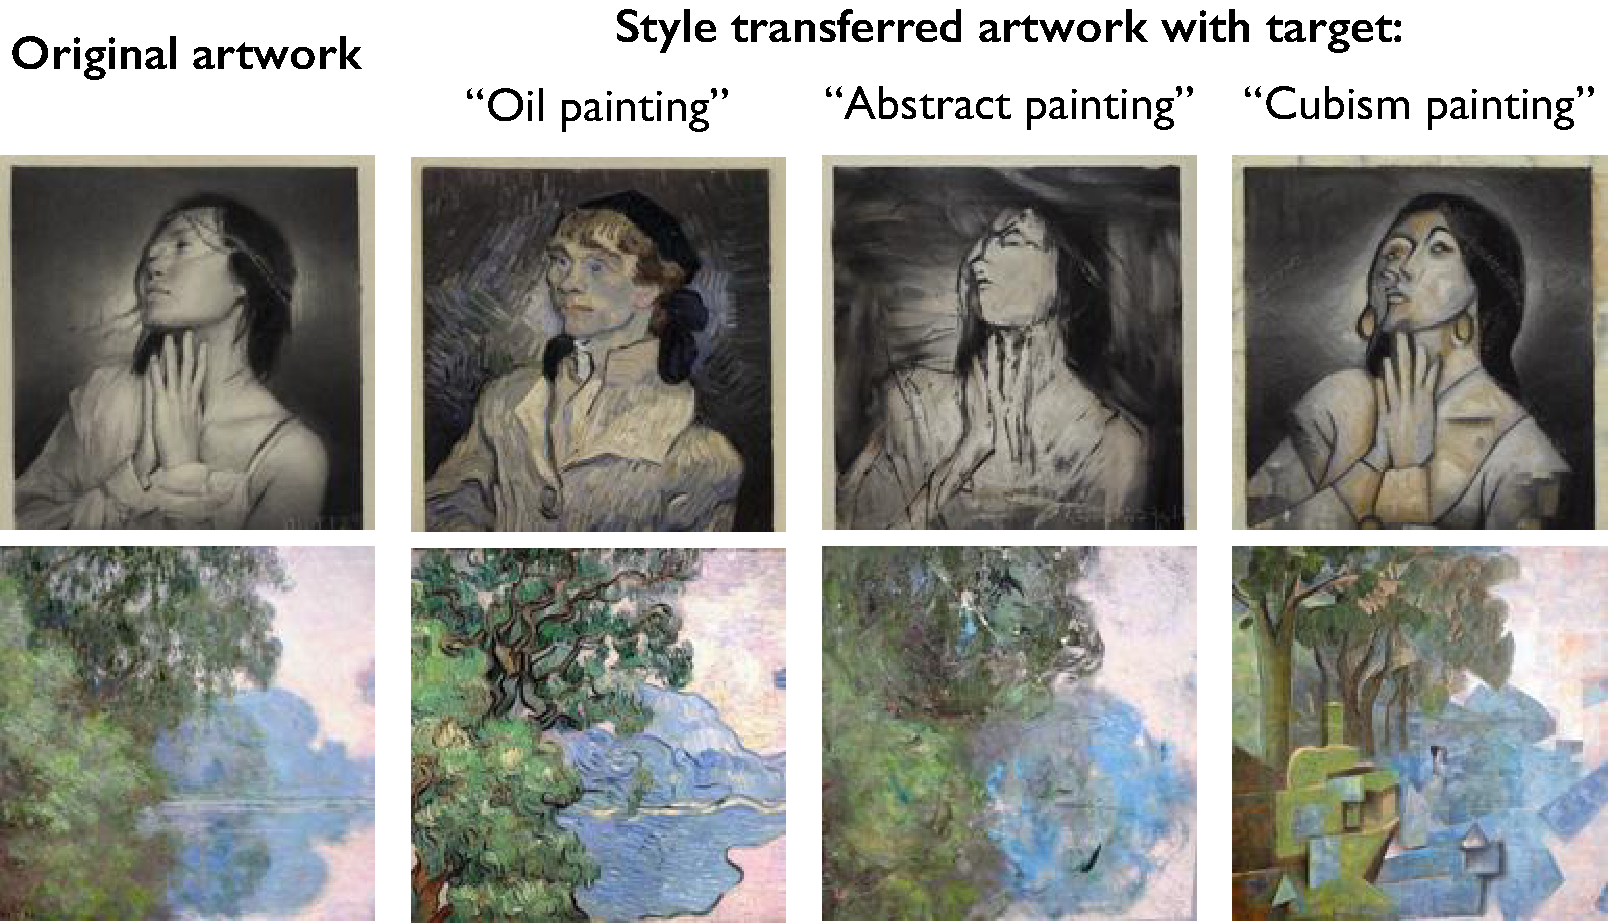
\includegraphics[width=1\columnwidth]{plots/eval/style-transfer-example.pdf}
  \caption{Example style-transferred artwork with different target styles. }
  \label{fig:transfer-examples}
\end{figure}

\secspace
\section{Disrupting Style Mimicry with Glaze} 
\label{sec:design}

In this section, we introduce \system{}, its design intuition followed by the
detailed algorithm. 

\secspace
\subsection{Design Intuition}
\label{sec:intuition-cloak}

Our key intuition is to identify and isolate \textit{style-specific features}
of an artist's original artwork, \ie the set of image features that
correspond to artistic style. Then \system{} computes cloaks while focusing
the perturbation budget on these style-specific features to maximize impact
on stylistic features.

As discussed, identifying and calculating style-specific features in model's
feature space is difficult due to the poor interpretability of model features
and how art style manifests differently across artworks. We overcome these two
challenges by designing a style-dependent and artwork-dependent method that
operates at image space. Given an artwork, we leverage ``style transfer,'' an
end-to-end computer vision technique, to modify and isolate its style
components. ``Style transfer'' transforms an image into a new image with a
different style (\eg from impressionist style to cubist style) while keeping
other aspects of the image similar (\eg subject matter and location).
% This is ideal for our use case, where protection must focus
% on style-specific features.

We leverage style transfer in our protection technique as follows. Given an
original artwork from the victim artist, we apply style-transfer to produce a
similar piece of art with a different style, \eg in style of ``an oil
painting by Van Gogh'' (Figure~\ref{fig:cloak-intuition} a). The new
version has similar content to the original, but its style mirrors that
of Van Gogh. We show more style-transfer examples with different target styles in
Figure~\ref{fig:transfer-examples}. Now, we can use the style-transferred
artwork as projection target to guide the perturbation computation. This
perturbs the original artwork's style-specific features towards that of
the style-transferred version. We do this by optimizing a cloak that, when
added to the original artwork, makes its feature representation similar to
the style-transferred image. Since the content is identical between the pair
of images, cloak optimization will focus its perturbation budget on style
features. 

\secspace
\subsection{Computing Style Cloaks} 

Using this approach, we compute style cloaks to disrupt style mimicry as
follows. Given an artwork ($x$), we use an existing feature extractor to
compute the style-transferred version of $x$ into target style $T$: $\Omega(x, T)$.
%style-transfer neural network that style transfers image $x$ and outputs
We then compute a style cloak $\delta_x$, such that $\delta_x$ moves $x$'s
style-specific feature representation to match that of $\Omega(x, T)$ while
minimizing visual impact. The cloak generation optimization is:

\secspace
\begin{eqnarray}
   &\min\limits_{\delta_x} Dist\left( \Phi(x + \delta_x), \Phi (\Omega(x, T))\right),  \label{eq:cloakopt}\\
  & \text{subject to } \; |\delta_x|< p, \nonumber
\end{eqnarray} 

\noindent where $\Phi$ is a generic image feature extractor commonly used in
text-to-image generation tasks, $Dist(.)$ computes the distance of two
feature representations, $|\delta_x|$ measures the perceptual perturbation
caused by cloaking, and $p$ is the perceptual perturbation budget. 

As discussed in \S\ref{sec:intuition-cloak}, the use of the style-transferred
image $\Omega(x, T)$ guides the cloak optimization in Eq~(\ref{eq:cloakopt})
to focus on changing style-specific image features. To maximize cloak
efficacy, the target style $T$ should be dissimilar from artist's original
style in the feature space. We discuss our heuristic for selecting target styles in
\S\ref{sec:design}.

\secspace
\subsection{Detailed System Design}
\label{sec:design-details}

Now we present the detailed design of \system{}. Given a victim
artist $V$, \system{} takes as input the set of $V$'s artwork to be shared
online $X_V$, an image feature extractor $\Phi$, a style-transfer model
$\Omega$, and perturbation budget $p$. Note that in many cases, a single
model (e.g. Stable Diffusion) provides both $\Phi$ and $\Omega$.

\para{Step 1: Choose Target Style.}  The selected target style $T$
should be sufficiently different from $V$'s style in model feature space to
maximize chances of disrupting style mimicry. For example, Fauvism and
Impressionism are distinct art styles that often look visually similar to the
untrained eye. Image of an impressionist painting style cloaked to Fauvism
might not produce a visually discernible effect on model-generated
paintings. Note that an artist can maximize their ability to avoid mimicry if
they consistently style cloak all their artwork towards the same target $T$.

For a new user, \system{} uses the following algorithm to randomly select $T$ from a set
of candidate styles reasonably different from $V$'s style. The algorithm
first inspects a public dataset of artists, each with a specific style (\eg
Monet, Van Gogh, Picasso). For each candidate target artist/style, it selects
a few images in that style and calculates their feature space centroid using
$\Phi$. It also computes $V$'s centroid in $\Phi$ using $V$'s artwork. Then,
it locates the set of candidate styles whose centroid distance to $V$'s
centroid is between the $50$ to $75$ percentile of all candidates. Finally,
it randomly selects $T$ from the candidate set.

\para{Step 2: Style transfer. } \system{} then leverages a pre-trained
style-transfer model $\Omega$~\cite{rombach2022high} to generate the
style-transferred artwork for optimization. Given each art piece $x \in
X_V$ and target style $T$, it style transfers $x$ to target style $T$ to
produce style-transferred image $\Omega(x, T)$.  

\para{Step 3: Compute cloak perturbation.} Then, \system{} computes the
cloak perturbation, $\delta_x$ for $x$, following the optimization defined
by eq. (\ref{eq:cloakopt}), subject to $|\delta_x| < p$. Our implementation
uses LPIPS (Learned Perceptual Image Patch
Similarity)~\cite{zhang2018unreasonable} to bound the perturbation. Different
from the $L_p$ distance used in previous
work~\cite{carlini2017towards,kurakin2016adversarial,sabour2015adversarial},
LPIPS has gained popularity as a measure of user-perceived image
distortion~\cite{cherepanova2021lowkey,laidlaw2020perceptual,rony2021augmented}. Bounding
cloak generation with this metric ensures that cloaked versions of images are
visually similar to the originals. We apply the \textit{penalty
  method}~\cite{nocedal2006numerical} to solve the optimization in
eq.(\ref{eq:cloakopt}) as follows:  

\vspace{-0.05in}
\begin{equation} \label{eq:optdetail} \vspace{-0.03in} 
 \underset{\delta_x}{\text{min }}||\Phi(\Omega(x, T)), \Phi(x + \delta_x) ||_2^2 + \alpha \cdot max(LPIPS(\delta_x)-p, 0) 
\end{equation}

\noindent where $\alpha$ controls the impact of the input perturbation. $L_2$
distance is used to calculate feature space distance.

\para{Upload artwork online.} Finally, the artist posts the cloaked artwork
online. For artists already with a large online presence, they can cloak and
re-upload artwork on their online portfolio.
While updating online images is not always possible, 
\system{} can be effective even when the mimic's model has significant amount
of uncloaked art (\S\ref{sec:robust-eval}).

\secspace
\subsection{On the Efficacy of Style Cloaks}
\label{sec:cloak-effect}

\system's style cloaks work by shifting feature representation of artwork in
the generator model. But how much shift do we need in order to have a
noticeable impact on mimicked art?


Two reasons suggest that even small shifts in style will have a meaningful
impact in disrupting style mimicry. First, generative models used for style
mimicry have {\em continuous} output spaces, \ie any shift in image feature
representation results in changes in the generated image.  Because generative
models are trained to interpolate their continuous feature
spaces~\cite{white2016sampling,upchurch2017deep}, any shift in the model's
representation of art style results in a new style, a ``blend'' between the
artist and the chosen target style.  
% the cloaked image with an \textbf{in-between style}, \ie a blended style of
% the original and target style,
Second, mimicked artwork must achieve reasonable quality and similarity in
style to the artist to be useful. Small shifts in the style space often
produce incoherent blends of conflicting styles that are enough to disrupt
style mimicry, \eg thick oil brushstrokes of Van Gogh's style mixed into a realism portrait.

These two factors contribute to \system{}'s success in more challenging
scenarios (\S\ref{sec:robust-eval}), and its robustness against
countermeasures (e.g. adversarial training) that succeed against cloaking
tools for facial recognition (\S\ref{sec:counter}).


\section{Evaluation}
\label{sec:eval-cloak}

In this section, we evaluate \system's efficacy in protecting artists from
style mimicry. We first describe the datasets, models, and experimental
configurations used in our tests. Then we present the results of \system's
protection in a variety of settings. Due to \system's highly visual nature,
we evaluate its performance using both direct visual assessment by
\textbf{human artists} in a user study, and \textbf{automated metrics} (see
\S\ref{sec:metrics} for details).

\para{Summary of results.} Over $93\%$ of artists surveyed believe \system{}
effectively protects artists' styles from AI style mimicry
attacks. Protection efficacy remains high in challenging settings, like when
the mimic has access to unprotected artwork. \system{} also achieves high
protection performance against a real-world mimicry-as-a-service platform. Of
our $1156$ artist participants, over $92\%$ found the perturbations
introduced by cloaking small enough not to disrupt the value of their art,
and over $88\%$ would like to use \system{} to protect their own artwork from
mimicry attacks.

\secspace
\subsection{Experiment Setup}
\label{sec:cloak-setup}

\para{Mimicry dataset. } We evaluate \system's performance in protecting the styles of the following two groups of artists: 

\vspace{-0.2cm}
\begin{packed_itemize}
\item {\em Current artists}: $4$ professional artists let us use their
  artwork in our experiments. These artists have different styles and
  backgrounds (\eg full-time/freelancers, watercolor painters/digital
  artists, well-known/independent). Each provided us with between $26$ to
  $34$ \textit{private} original art pieces for our experiments. We use
  perceptual hashing~\cite{ke2004efficient} to verify that none of these are
  included in existing public datasets used to train generic text-to-image
  models (e.g.~\cite{schuhmann2022laion,changpinyo2021conceptual}).  

\item {\em Historical artists}: We also evaluate \system{}'s protection on
  $195$ historical artists (\eg van Gogh, Monet) from the WikiArt
  dataset~\cite{saleh2015large}. The WikiArt dataset contains 42,129 art
  pieces from $195$ artists. Each art piece is labeled with its genre (\eg
  impressionism, cubism). We randomly sampled $30$ art pieces from each
  artist to use in style mimicry attacks. Generic text-to-image models found
  online have been trained on some artwork from these artists. Using this art
  simulates a more challenging scenario in which a famous artist attempts
  to disrupt a model that already understands their style.
\end{packed_itemize}
\vspace{-0.2cm}

\para{Mimicry attack setup. } We recreate the strongest-possible mimicry
attack scenario, based on techniques used in real-world mimicry
incidents~\cite{ruiz2022dreambooth,sam-steal,hollie-steal},
that works as follows. First, we take art pieces from the victim artist $V$
and generate a text caption for each piece using an image captioning
model~\cite{luo2022vc}. \revise{The pretrained image captioning model generates a short 
sentence to describe the image. We found that this model can correctly caption protected images (examples in Figure~\ref{fig:data-examples}), likely because \system{} focuses on perturbing style features while the captioning models focus on image content.} Then, we append the artist's name to each caption,
\eg ``mountain range \textit{by Vincent van Gogh}''. Finally, we fine-tune a pre-trained generic text-to-image model
(details below) on the caption/image pairs. 

We use $80\%$ of the art pieces from the victim artists to fine-tune models
that mimic each artist's style, reserving the rest for testing. We fine-tune
for $3000$ optimization steps, which we find achieves the best mimicry
performance (Figure~\ref{fig:success-iter} in Appendix). We then use the
fine-tuned, style-specific model to generate mimicked artwork in style of
each victim artist. We query the model using the generated captions (which
include $V$'s name) from the held-out test artwork set. We generate $5$
pieces of mimicked art for each text caption using different random seeds and
compare these to the real victim art pieces with this caption. Additional
details on training and generation parameters, as well as its sensitivity to
random seed selection and the number of training art pieces are in Appendix~\ref{app:mimicry}.  

% Fine-tuning a style-specific mimicry model takes 56.4 minutes on average on one Titan RTX GPU~\footnote{This takes longer than real-world mimicry incidents because we finetune more steps for better mimicry performance.}. 

\para{Text-to-image models.} We use two state-of-the-art, public, generic text-to-image models in our experiments: 

\vspace{-0.2cm}
\begin{packed_itemize}
\item \textit{Stable Diffusion (SD)}: Stable Diffusion is a popular and
  high-performing open-source text-to-image model~\cite{stable2-1},trained
  on 11.5 million images from the LAION dataset~\cite{schuhmann2022laion}. SD
  training takes over 277 GPU months (on A100 GPU) and costs around
  \$600K~\cite{stable2-1}. SD uses diffusion methods to generate images and
  achieves state-of-the-art performance on several
  benchmarks~\cite{rombach2022high}. Viewed as one of the best open-source
  models, SD has powered many recent developments in text-to-image
  generation~\cite{blender-plugin,novelai-update,gimp,aigame}. We
  use SD version 2.1 in the paper~\cite{stable2-1}, the most up-to-date
  version as of December 2022.  

\item \textit{DALL$\cdot$E-mega (\dalleM)}: \dalleM-mega, an updated version
  of the more well-known \dalleM-mini, is an open-source model based on
  OpenAI's \dalleM~1~\cite{ramesh2021zero}. The model leverages a VAE for
  image generation and is trained on 17 million images from three different
  datasets~\cite{sharma-etal-2018-conceptual,changpinyo2021conceptual,thomee2016yfcc100m}. Training
  takes 2 months on 256 TPUs~\cite{mini-training}. While \dalleM~ performs
  worse than diffusion-based models like SD, we use it to evaluate how
  \system~generalizes to different model architectures.  
\end{packed_itemize}

\vspace{-0.2cm}

\para{\system~configuration. } We generate cloaks for each of victim $V$'s
art pieces following the methodology of \S\ref{sec:design-details}. First, we
use the target selection algorithm to select a target style $T$. We choose
from a set of $1119$ candidate target styles, collected by querying the
WikiArt dataset with artist and genre names, \eg ``Impressionism painting by
Monet''~\footnote{One artist may paint in multiple styles, resulting in
  multiple candidate target styles from a single artist.}. We then style
transfer each victim art piece into the target style leveraging the style
transfer functionality of stable diffusion model (stable diffusion model has
both text-to-image and style transfer functionality). \revise{A style transfer model takes
in an original image and a target prompt as input. Leveraging a similar diffusion process, the model
modifies the original image to a style similar to that described in the target prompt. More information on style transfer can be found in ~\cite{saharia2022palette}}. Finally, we optimize a cloak for each art piece
using Eq.~\ref{eq:optdetail} by running the Adam optimizer for $500$
steps. \revise{We benchmark \system{}'s runtime on artwork with resolution ranging 
from $512$ to $6000$ pixels, using SD's feature extractor (ViT model with 83 million parameters). } It takes an average of $1.2$ mins on Titan RTX GPU and $7.3$ mins on a
single Intel i7 CPU to generate a cloak for a single piece of art. 

In our initial experiments, we assume \system{} generates cloaks using the
same image feature extractor as the mimic (e.g. SD's or \dalleM's feature
extractor). We relax this assumption and evaluate
\system{}'s performance when artists and mimics use different feature
extractors in \S\ref{sec:robust-eval}.

\secspace
\subsection{Evaluation Metrics} 
\label{sec:metrics}

We evaluate our protection performance using both visual assessment and feedback from
human artists, and a scalable metric. Here, we describe the setup of our
evaluation study and define the exact metrics used for evaluation.  

% \vspace{-0.2cm}
% \begin{packed_itemize}
\para{Artist-rated protection success rate (Artist-rated PSR): } The user
studies ask artists to rate the performance of \system. We generate a dataset
of mimicry attacks on $13$ victim artists (the $4$ current artists and $9$
randomly chosen historical artists) across $23$ protection scenarios
(including ones in \S\ref{sec:counter}). For each participant, we randomly
select a set of mimicry attacks out of these $13 \times 23$ settings and ask
them to evaluate protection success.  For each mimicry attempt, we show
participants $4$ mimicked art pieces and $4$ original art pieces from the
victim artist. \revise{Using original art pieces as an indicator of the human
artist's style,} we ask participants to consider the mimicked art, and rate the success of 
\system{}'s
protection on a 5-level Likert scale (ranging from ``not successful at all''
to ``very successful''). Each mimicry attempt is evaluated by at least $10$
participants. We define \textit{artist-rated PSR} as the percent of
participants who rated \system{}'s protection as ``successful'' or ``very
successful.''  Our user studies primarily focus on artists, as they would be
most affected by this technology. We found though, that not all current
artists despise AI art, and some view it as a new avenue for a different form
of artistry.

\para{CLIP-based genre shift: } We define a new metric based on
CLIP~\cite{radford2021learning}, using the intuition that \system{} succeeds
if the mimicked art has been impacted enough by \system{} to be classified
into a \textit{different art genre} from the artist's original artwork. We
leverage CLIP model's ability to classify art images into art genres. Given a
set of mimicked art targeting an artist $V$, we define \textit{CLIP-based
  genre shift rate} as the percentage of mimicked art whose top 3 predicted
genres do not contain $V$'s original genre. A higher genre shift rate means
more mimicked art belongs to a different genre from the victim artist, and thus
means more successful protection.

To calculate the genre shift we use a set of $27$ historical genres from
WikiArt dataset and $13$ digital art genres~\cite{digital-styles} as the
candidate output labels. In Appendix~\ref{app:clip}, we show that a
pre-trained CLIP model is able to achieve high genre classification
performance. We report the average CLIP-based genre shift for all 199 victim
artists across all mimicked artworks.

We use CLIP-based genre shift as a supplemental metric to evaluate \system{}
because it is only able to detect style changes at the granularity of art
genres.
% checks whether the mimicked artwork belongs to a different
% art genre as artist's true genre.
However, mimicry attacks also fail when
\system{} causes the mimicked artwork quality to be very low, something that 
CLIP cannot measure. Measuring the quality of generated image has been a
challenging and ongoing research problem in computer
vision~\cite{kynkaanniemi2022role,blau2018perception,karras2020training}.


\begin{figure*}[t]
  \centering
  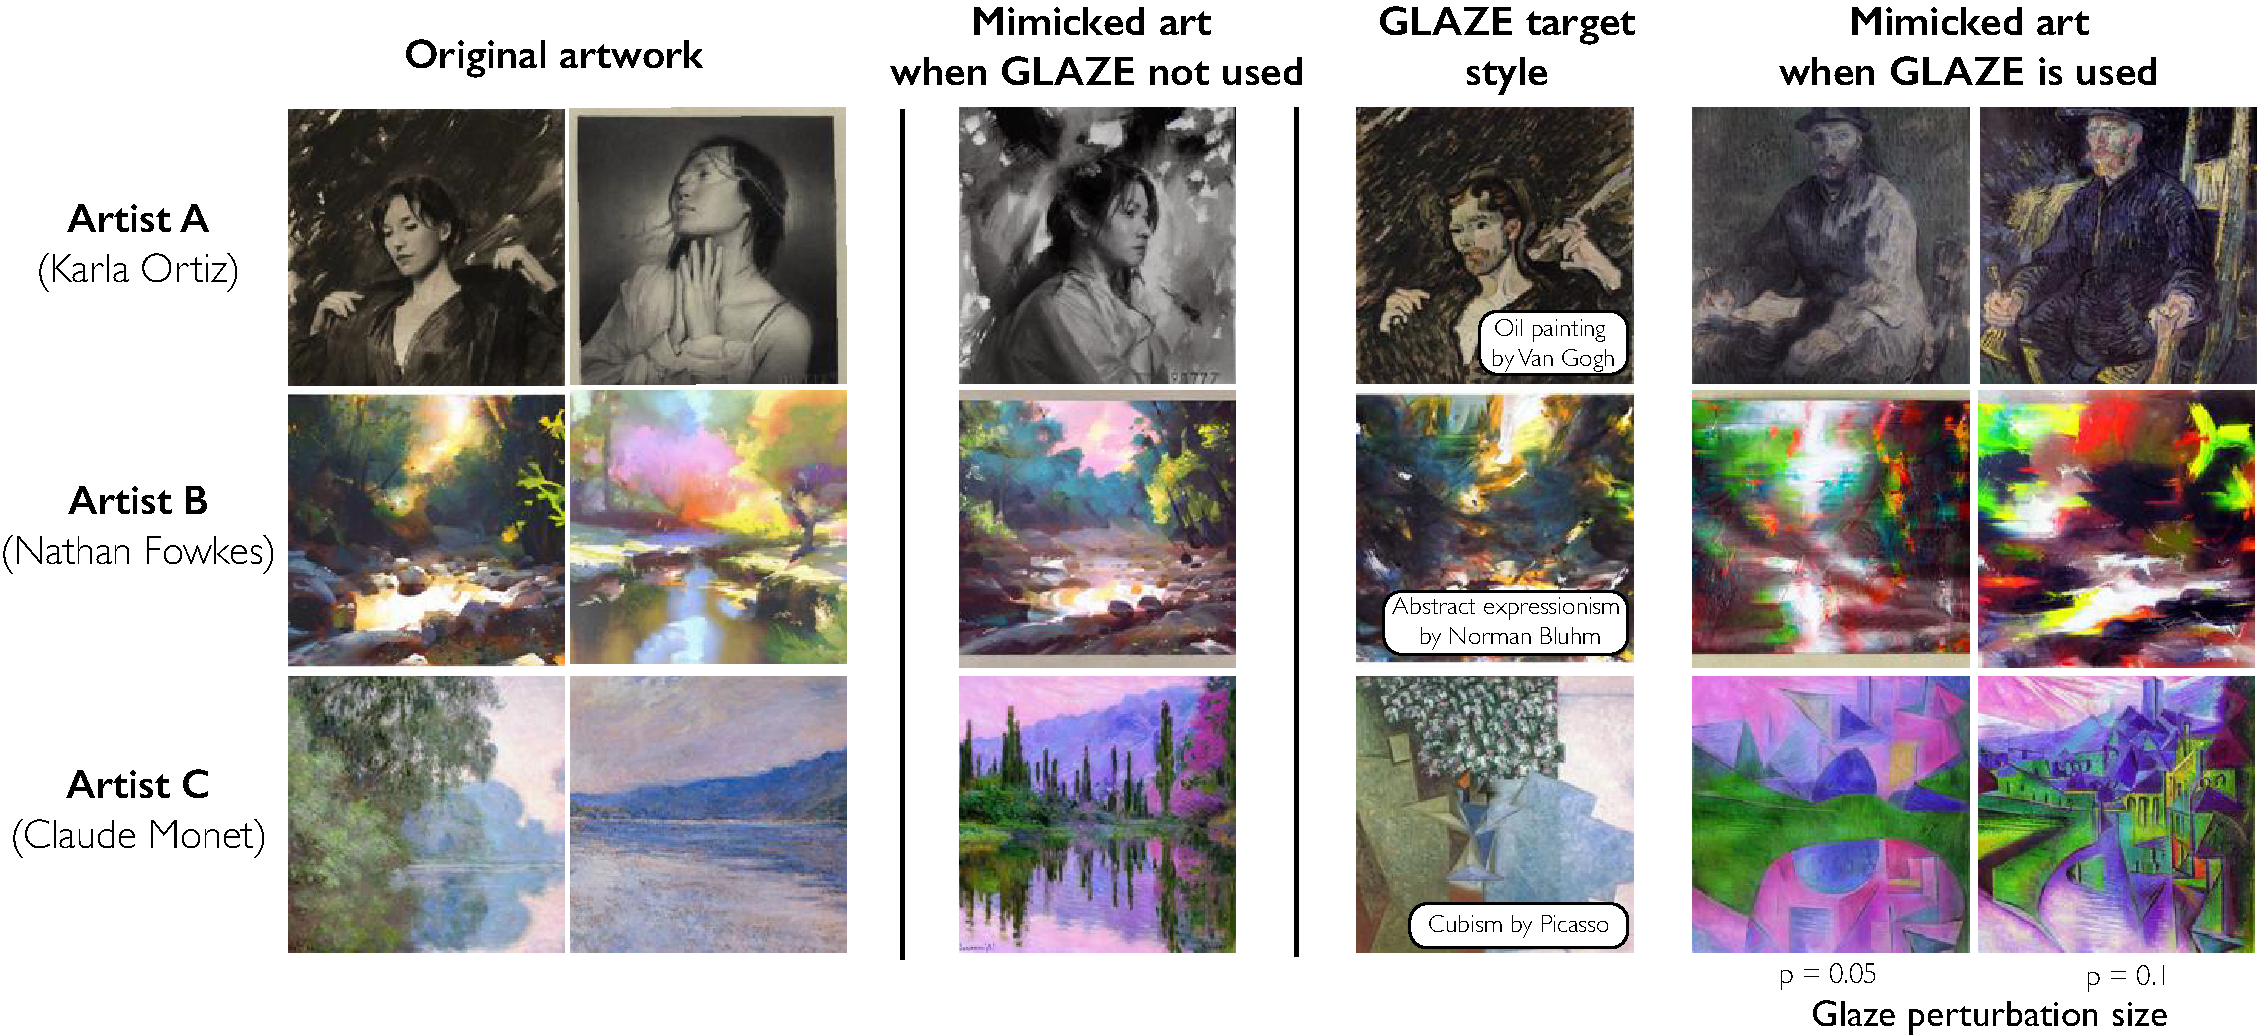
\includegraphics[width=0.9\linewidth]{plots/eval/big-result-full-emily.pdf}
  \vspace{-0.1in}
  \caption{Example \system{} protection results for three artists. {\bf
      Columns 1-2}: artist's original artwork; {\bf column 3}: mimicked
    artwork when artist does not use protection; {\bf column 4}:
    style-transferred artwork (original artwork in column 1 is the source)
    used for cloak optimization and the name of target style; {\bf column
      5-6}: mimicked artwork when artist uses cloaking protection with
    perturbation budget $p=0.05$ or $p=0.1$ respectively. All mimicry
    examples here use SD-based models.
  } %The images can be zoomed for a closer look when viewing the paper digitally. )}
  \label{fig:core-res}
\end{figure*}

\begin{table}[t]
  \centering
  \resizebox{0.5\textwidth}{!}{
  \centering
\begin{tabular}{cccccc}
\toprule
\multirow{2}{*}{\textbf{\begin{tabular}[c]{@{}c@{}} \\ Generic \\ model\end{tabular}}} & \multirow{2}{*}{\textbf{\begin{tabular}[c]{@{}c@{}}\\ Artist \\ dataset\end{tabular}}} & \multicolumn{2}{c}{\textbf{w/o \system{}}} & \multicolumn{2}{c}{\textbf{w/ \system{} (p=0.05)}} \\ \cmidrule{3-6} 
 &  & \begin{tabular}[c]{@{}c@{}}Artist-rated \\ PSR\end{tabular} & \begin{tabular}[c]{@{}c@{}}CLIP-based \\ genre shift\end{tabular} & \begin{tabular}[c]{@{}c@{}}Artist-rated \\ PSR\end{tabular} & \begin{tabular}[c]{@{}c@{}}CLIP-based \\ genre shift\end{tabular} \\ \midrule
\multirow{2}{*}{SD} & Current & $4.6 \pm 0.3\%$ & $2.4 \pm 0.2\%$ & $94.3 \pm 0.8\%$ & $96.4 + 0.5\%$ \\
 & Historical & $4.2 \pm 0.2\%$ & $1.3 \pm 0.2\%$ & $93.3 + 0.6\%$ & $96.0 + 0.3\%$ \\ \midrule
\multirow{2}{*}{\dalleM~} & Current & $31.9 \pm 3.5\%$ & $6.4 \pm 0.8\%$ & $97.4 \pm 0.2\%$ & $97.4 + 0.3\%$ \\
 & Historical & $29.8 \pm 2.4\%$ & $5.8 \pm 0.6\%$ & $96.8 \pm 0.3\%$ & $97.1 + 0.2\%$ \\ \bottomrule
\end{tabular}
  }
  \vspace{-0.1in}
  \caption{\system{} has a high protection success rate, as measured by
    artists and CLIP, against style mimicry attacks. We compare protection
    success when artists do not use \system{} vs. when they do (with
    perturbation budget 0.05). }
  \label{tab:psr-core-table}
  \vspace{-0.3cm}
\end{table}

\begin{figure*}[t]
  \centering
  \begin{minipage}{0.32\textwidth}
  \centering
  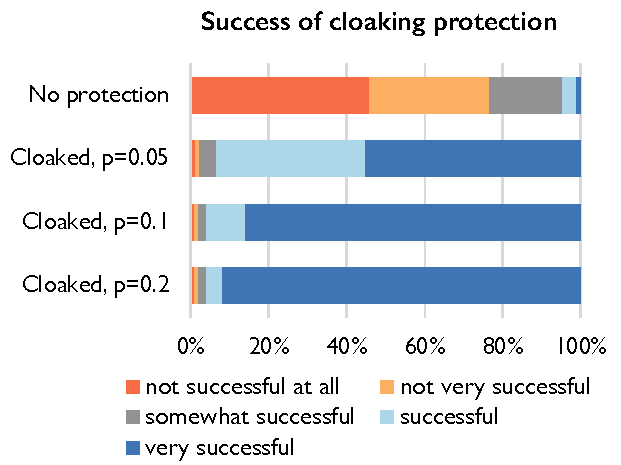
\includegraphics[width=1\columnwidth]{plots/eval/user-cloak-budget.pdf}
  \vspace{-0.23in}
  \caption{\system{}'s cloaking protection success increases as cloak perturbation budget increases. The top row of the figure shows baseline performance with the mimic trains on uncloaked images (p=0). }
  \label{fig:budget-increase}
  \end{minipage}
  \hfill
    \centering
    \begin{minipage}{0.32\textwidth}
  \vspace{0.23in}
  \centering
    \resizebox{1\textwidth}{!}{
    \begin{tabular}{lcc}
    \toprule
    \multicolumn{1}{c}{\textbf{\begin{tabular}[c]{@{}c@{}}Perturbation\\ budget\end{tabular}}} & \textbf{\begin{tabular}[c]{@{}c@{}}Artist-rated \\ PSR\end{tabular}} & \textbf{\begin{tabular}[c]{@{}c@{}}CLIP-based \\ genre shift\end{tabular}} \\ \midrule
    0 (no cloak) & $4.6 \pm 1.4\%$ & $2.4 \pm 0.8\%$ \\
    0.05 & $93.3 \pm 0.6\%$ & $96.0 \pm 0.3\%$ \\
    0.1 & $95.9 \pm 0.4\%$& $98.2 \pm 0.1\%$ \\
    0.2 & $96.1 \pm 0.3\%$ & $98.5 \pm 0.1\%$ \\ \bottomrule
    \end{tabular}
    }
    \vspace{0.13in}
    \captionof{table}{Performance of our system (artist-rated protection success rate and CLIP-based genre shift rate) increases as the perturbation budget increases. (SD model, averaged over all victim artists). }
    \label{tab:budget-increase-sd}
  \end{minipage}
  \hfill
\centering
  \begin{minipage}{0.32\textwidth}
  \centering
  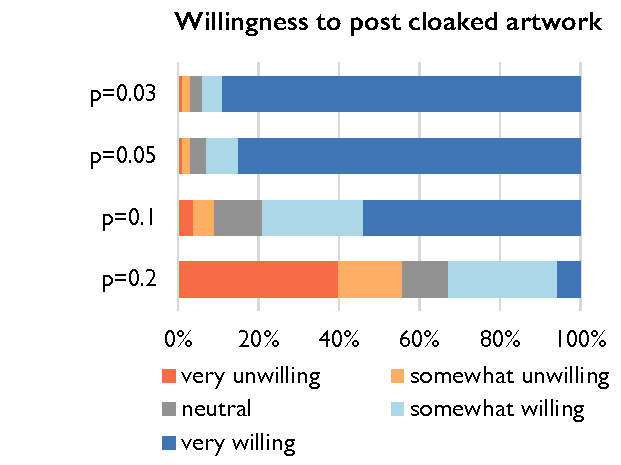
\includegraphics[width=1\columnwidth]{plots/eval/user-accept.pdf}
  \vspace{-0.23in}
  \caption{Artists' willingness to post cloaked artwork in place of the original decreases as perturbation budget of the cloaks increases. }
  \label{fig:artist-accept} 
  \end{minipage}
    \hfill
\end{figure*}

\begin{figure}[t]
  \centering
  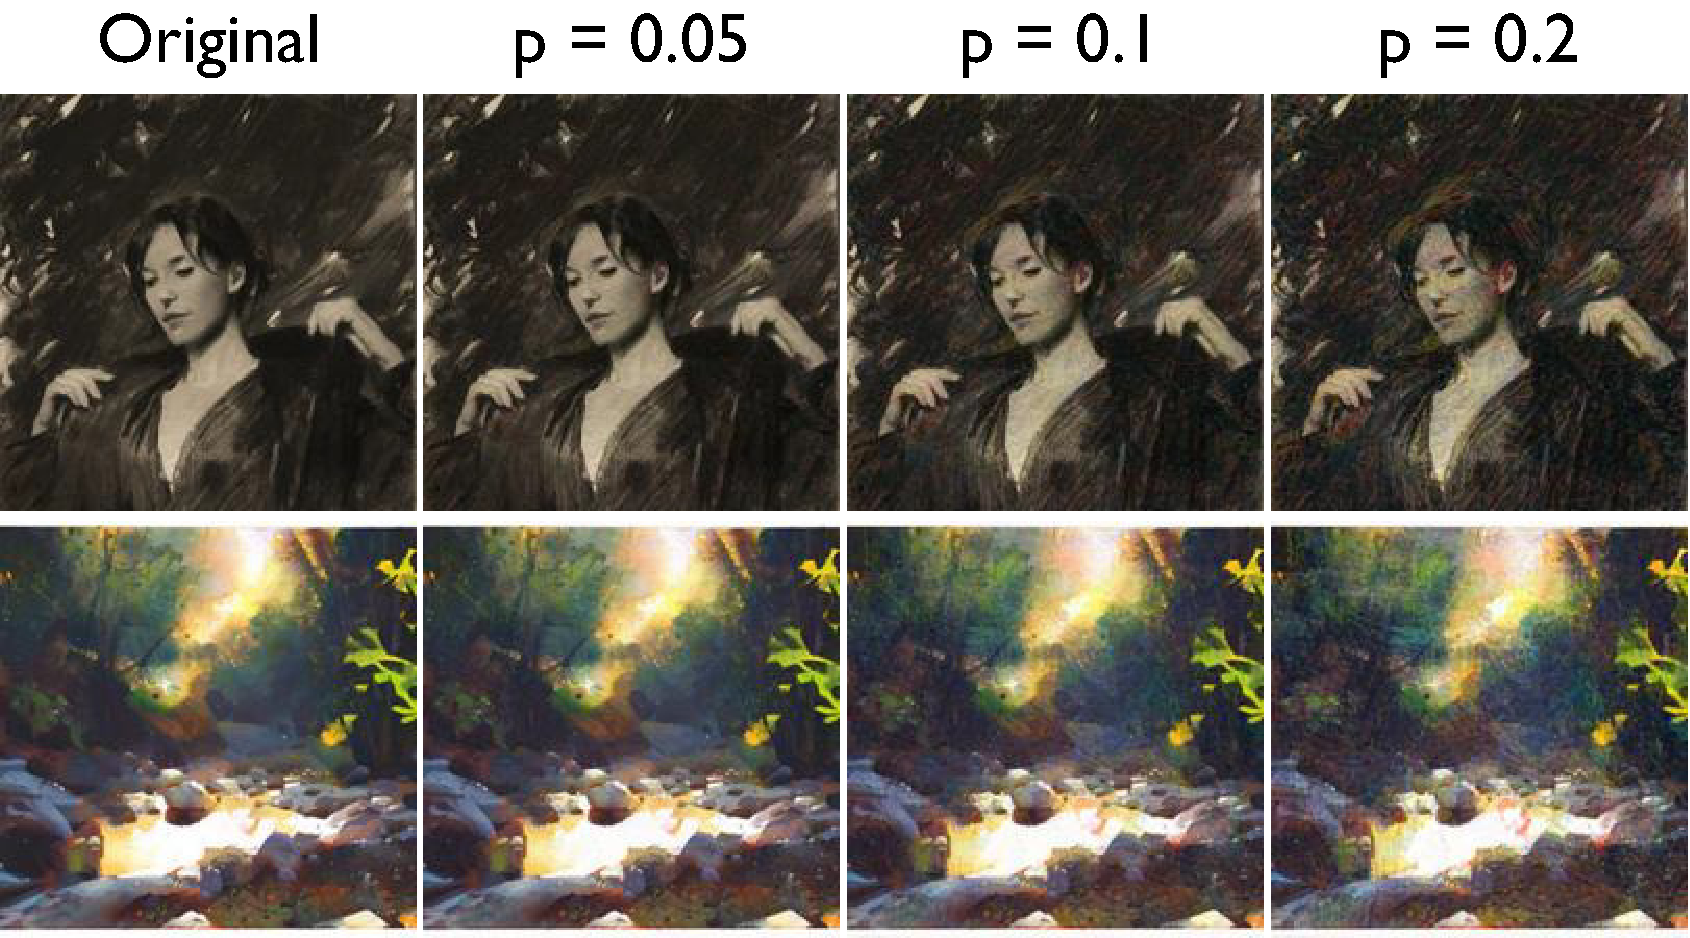
\includegraphics[width=0.90\columnwidth]{plots/eval/cloak-perturbation.pdf}
  \vspace{-0.08in}
  \caption{Original artwork and cloaked artwork computed using three different cloak perturbation budgets. }
  \label{fig:before-after}
\end{figure}

\secspace
\subsection{\system{}'s Protection Performance}
\label{sec:cloaking-results}

\para{Style mimicry success when \system{} is not used. } Mimicry attacks are
very successful when the mimic has access to a victim's original (unmodified)
artwork. Examples of mimicked artwork can be found in
Figure~\ref{fig:core-res}. The leftmost two columns of Figure~\ref{fig:core-res} show a
victim artist's original artwork, while the third column depicts mimicked
artwork generated by a style-specific model trained on victim's original
artwork when \system{} is not used. In our user study, over $>95\%$ of
respondents rated the attack as successful. Table~\ref{tab:psr-core-table},
row 1, gives the artist-rated and CLIP-based genre shift for mimicry attacks on
unprotected art. 

SD models produce stronger mimicry attacks than \dalleM{} models, according
to our user study (see Table~\ref{tab:psr-core-table}). This is unsurprising,
as \dalleM{} models generally produce lower-quality generated
images. CLIP-based genre shift does not reflect this phenomenon, as this metric does
not assess image quality.  

\para{\system{}'s success at preventing style mimicry. } \system{} makes
mimicry attacks markedly less successful, as shown in
Figure~\ref{fig:core-res}. Columns 5 and 6 (from left) show mimicked artwork
when the style-specific models are trained on artwork protected by
\system{}. For reference, column 4 shows an example style-transferred artwork
$\Omega(x, T)$ used to compute \system{} cloaks for the protected art
pieces. Overall, \system{} achieves $> 93.3\%$ artist-rated PSR and
$> 96.0\%$ CLIP-based genre shift (see Table~\ref{tab:psr-core-table}). \system{}'s
protection performance is slightly higher for current artists than for
historical artists. This is likely because the historical artists' images are
present in the training datasets of our generic models (SD, \dalleM),
highlighting the additional challenge of protecting well-known artists whose
style was already learned by the generic models.

\para{How large of perturbations will artists tolerate?} Increasing the
\system{} perturbation budget enhances protection performance. We observe
that both artist-rated and CLIP-based genre shift increase with perturbation budget
(see Figure~\ref{fig:budget-increase}, Table~\ref{tab:budget-increase-sd},
and Figure~\ref{fig:budget2results}). Given this tradeoff between protection
success and \system{} protection visibility on original artwork, we evaluate
how perturbation size impacts artists' willingness to use \system{}. 

We find that artists are willing to add fairly large \system{} perturbations
to their artwork in exchange for protection against mimicry. To measure this,
we show $3$ randomly chosen pairs of original/cloaked artwork to each of the
1,156 artists in our first study. For each art pair, we ask the artist
whether they would be willing to post the cloaked artwork (instead of the
original, unmodified version) on their personal website. More than $92\%$ of
artists select ``willing'' or ``very willing'' when $p=0.05$. This number
only slightly increases to $94.3\%$  when $p=0.03$.
Figure~\ref{fig:artist-accept} details artists' preferences as perturbation
budget increases. (see Figure~\ref{fig:before-after} for examples of cloaked
artwork with increasing $p$). Based on these results, we use perturbation
budget $p = 0.05$ for all our experiments, since most artists are willing to
tolerate this perturbation size.  

Surprisingly, over $32.8\%$ artists are willing to use cloaks with $p=0.2$,
which is clearly visible to human eye (see Figure~\ref{fig:before-after}). While we
are surprised by this high perturbation tolerance, in our follow-up free
response artists noted that they would be willing to tolerate large
perturbations because of the devastating consequence if their styles are
stolen. One participant stated that ``I am willing to sacrifice a bit image
quality for protection.'' Many artists ($>80\%$) also noted that they have
already used traditional, more visually disruptive techniques to protect
their artwork online when posting online, \ie adding watermark or reducing
image resolution. One participant stated that ``I already use low to medium
resolution images only for online posting, thus this would not impact my
quality control too much.'' 

\begin{figure*}[t]
  \centering
  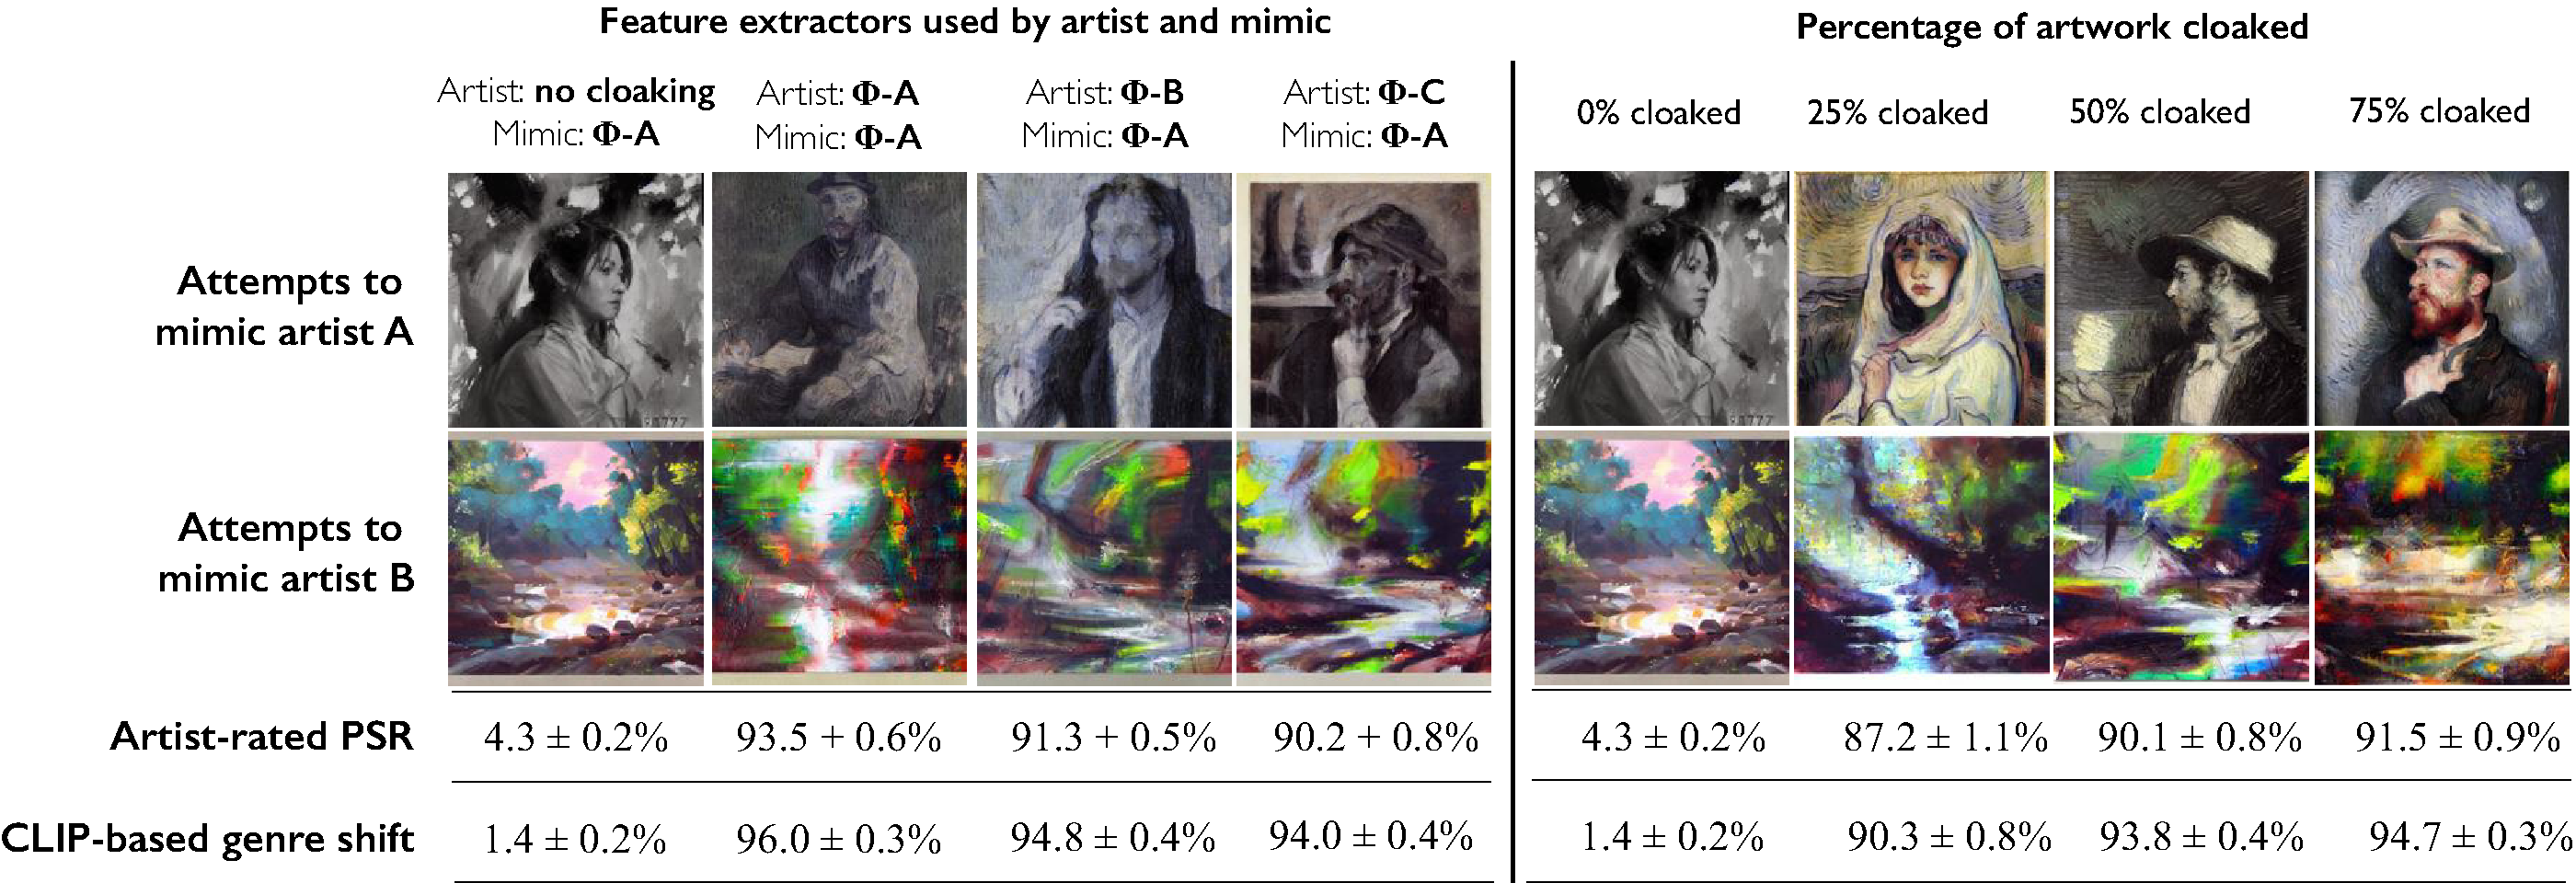
\includegraphics[width=0.95\linewidth]{plots/eval/eval-robust.pdf}
  \caption{\system{} remains successful under two challenging
    scenarios. Left: when artist and mimic use different feature
    extractors. Right: when artists can only cloak a portion of their artwork
    in mimic's dataset. Bottom of the figure shows artist-rated PSR and
    CLIP-based genre shift for the corresponding setting. } 
  \label{fig:core-robust}
\end{figure*}

\secspace
\subsection{\system{}'s Protection Robustness}
\label{sec:robust-eval}

\secspace

Next, we test \system{}'s efficacy in more challenging scenarios. First, we
measure performance when the mimic uses a different feature extractor for
mimicry than the one used by the artist to generate the cloak. Second, we
measure what happens when the mimic has uncloaked artwork samples from the
victim.  Due to the poor mimicry performance of \dalleM, we focus our
evaluation using SD as the generic model.

\para{Artist/mimic use different feature extractors. } In the real world, it
is possible that the mimic will use a different model (and thus a different image
feature extractor) for style mimicry than the one used by the victim artist
to cloak their artwork. While the feature extractors may still be similar
because of the well-known transferability property between large
models~\cite{demontis2019adversarial,transfer,suciu2018does,transfer2014,shan2022post},
their differences could reduce the efficacy of cloaking. We test this
scenario using three feature extractors\textemdash $\Phi$-A, $\Phi$-B, and
$\Phi$-C. $\Phi$-A and $\Phi$-B have different model architectures
(autoencoder-KL~\cite{rombach2022high} vs. VQ-VAE~\cite{ramesh2021zero}) but
are both trained on the ImageNet dataset~\cite{deng2009imagenet}. $\Phi$-A
and $\Phi$-C have different model architectures (autoencoder-KL vs VQ-VAE)
and training datasets (ImageNet vs. CelebA~\cite{liu2018large}).

In our experiments, the victim artist uses one feature extractor (either
$\Phi$-B or $\Phi$-C) to optimize cloaked artwork, and the mimic trains their
style-specific models with SD models using $\Phi$-A. Despite the difference
in victim/mimic extractors, \system{}'s protection remains highly successful
(left half of Figure~\ref{fig:core-robust})\textemdash the style of mimicked
artwork remains distinct from artist's true style. Artist-rated and
CLIP-based genre shift measurements confirm this observation. Artist-rated PSR is
$> 90.2\%$, while CLIP-based genre shift is $> 94.0\%$. The PSR is slightly higher
when the two feature extractors only differ in architectures ($\Phi$-B to
$\Phi$-A) than when they differ in both architecture and training data
($\Phi$-C to $\Phi$-A).


\para{Mimic has access to uncloaked artwork. } Another challenging scenario
is when the mimic gains access to some \textit{uncloaked} artwork from victim
artists. This is a realistic scenario for many prominent artists with a large
online presence. As expected, \system{}'s protection performance decreases
when the mimic has access to more uncloaked artwork (right side of
Figure~\ref{fig:core-robust}). As the ratio of uncloaked/cloaked art in the
mimic's dataset increases, the mimicked artwork becomes more similar to
artist's original style. Yet, \system{} is still reasonably effective
($87.2\%$ artist-rated PSR) even when artists can only cloak $25\%$ of their
artwork. This validates our hypothesis in \S\ref{sec:cloak-effect} that
cloaking will have a noticeable effect as long as the mimic has some cloaked
training data.

A mimic with access to a large amount of uncloaked artwork is still an issue
for \system{}. Fortunately, in our user study, we found that 1) many artists
constantly create and share new artwork online, which can be cloaked to
offset the percentage of uncloaked artwork, and 2) many artists change their
artistic style over time. In our user study, we asked artists to estimate the
number of unique art pieces they currently have online ($M$) and the
estimated number of art pieces they anticipate uploading each subsequent year
($Y$). Among artists with an existing online presence, over $40\%$ have
$Y / M > 25\%$, meaning that one year from now, $> 20\%$ of their total
online artwork would be cloaked (if they start using \system{}
immediately). More than $81\%$ of artists also stated that their art style
has changed over their career, and half of these said that theft of their
old, outdated styles is less concerning.


\begin{table}[t]
  \centering
  \resizebox{0.49\textwidth}{!}{
  \centering
  \begin{tabular}{ccccc}
    \hline
    \multirow{2}{*}{\textbf{\begin{tabular}[c]{@{}c@{}}Artist \\ dataset\end{tabular}}} & \multicolumn{2}{c}{\textbf{w/o \system}} & \multicolumn{2}{c}{\textbf{w/ \system{} (p=0.05)}} \\ \cline{2-5} 
     & \begin{tabular}[c]{@{}c@{}}Artist-rated \\ PSR\end{tabular} & \begin{tabular}[c]{@{}c@{}}CLIP-based \\ genre shift\end{tabular} & \begin{tabular}[c]{@{}c@{}}Artist-rated \\ PSR\end{tabular} & \begin{tabular}[c]{@{}c@{}}CLIP-based \\ genre shift\end{tabular} \\ \hline

    Current & $6.2 \pm 0.5\%$ & $3.8 \pm 0.3\%$ & $92.5 \pm 0.5\%$ & $94.2 + 0.3\%$ \\
    Historical & $7.2 \pm 0.6\%$ & $3.3 \pm 0.4\%$ & $92.1 + 0.3\%$ & $93.9 + 0.4\%$ \\ 
    \hline
    \end{tabular}
  }
  \vspace{-0.1in}
  \caption{Performance of \system{} against real-world mimicry service
    (scenario.gg). Mimicry service achieves high mimicry success when no
    protection is used. When \system{} is used, the mimicry service has low
    performance. }
  \label{tab:real-world}
\end{table}

\secspace
\subsection{Real-World Performance}

Next, we test \system{} against a real-world style mimicry-as-a-service
system, \texttt{scenario.gg}~\cite{aigame}. Scenario.gg is a web service that
allows users to upload a set of images in a specific style. The
service then trains a model to mimic the style and returns an API endpoint
that allows the user to generate mimicked images in the trained style. The
type of model or mimicry method used by the service is unknown.

\system{} remains effective against \texttt{scenario.gg}. We ask
\texttt{scenario.gg} to mimic the style from a set of cloaked or uncloaked
artwork from $4$ current artists and $19$ historical
artists. Table~\ref{tab:real-world} shows that when no protection is used,
\texttt{scenario.gg} can successfully mimic the victim style (< 7.2\%
protection success). The mimicry success of \texttt{scenario.gg} is lower
than our mimicry technique, likely because \texttt{scenario.gg} trains the
model for fewer iterations due to computational constraints. When we use
\system{} to cloak the artwork and upload the cloaked artwork,
\texttt{scenario.gg} fails to mimic the victim style ($> 92.1\%$ artist-rated
PSR and $> 93.9\%$ CLIP-based genre shift rate) as shown in Table~\ref{tab:real-world}.

\begin{figure}[t]
  \centering
  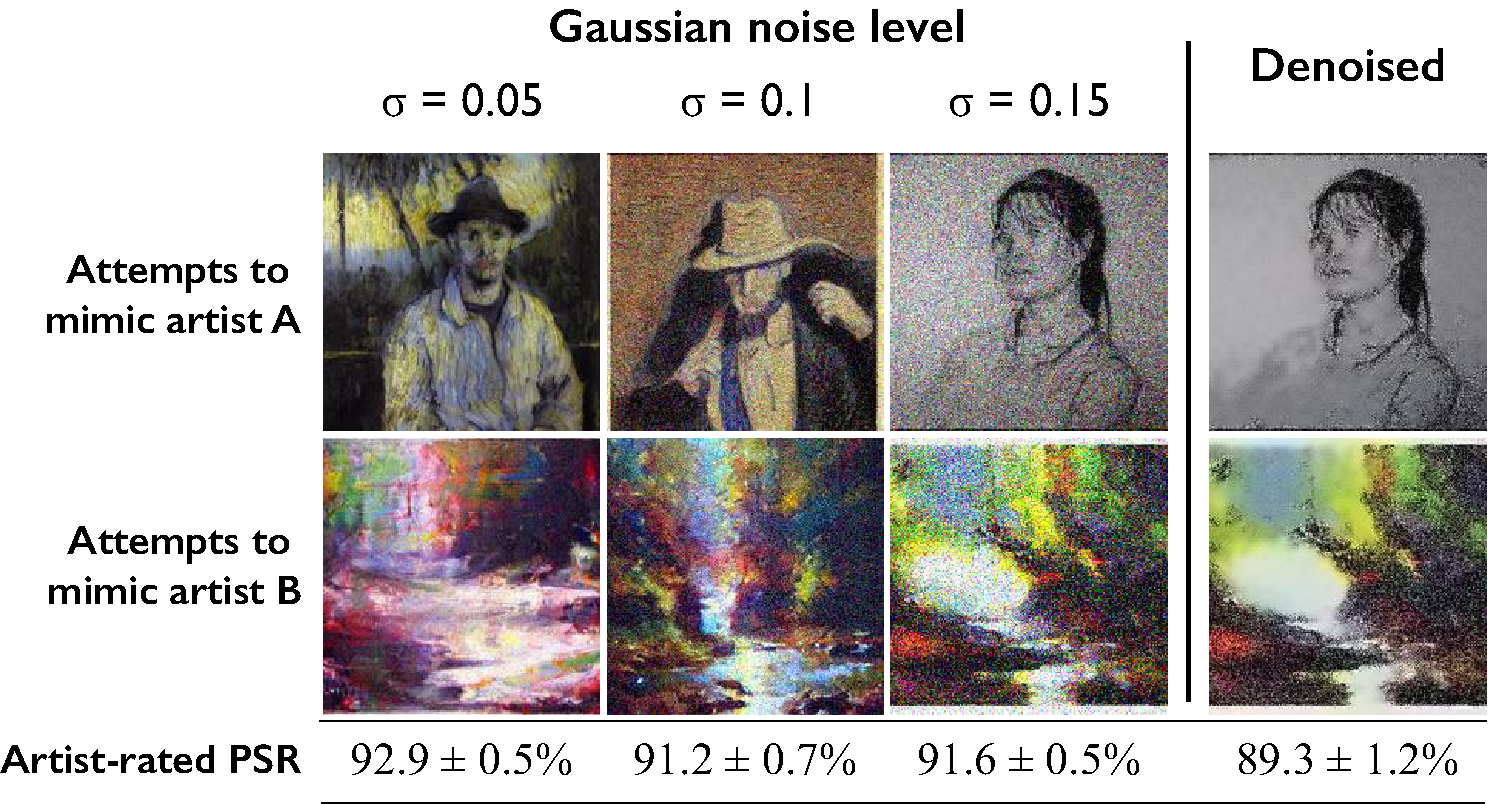
\includegraphics[width=1\columnwidth]{plots/counter/add-noise.pdf}
    \vspace{-0.25in}
  \caption{\system{}'s protection performance remains high as mimic adds an
    increasing amount of Gaussian noise to the cloaked artwork. Even when the
    mimic adds denoising (last column), \system{}'s protection persists. } 
  \label{fig:noise_countermeasure}
\end{figure}

\begin{figure}[t]
  \centering
  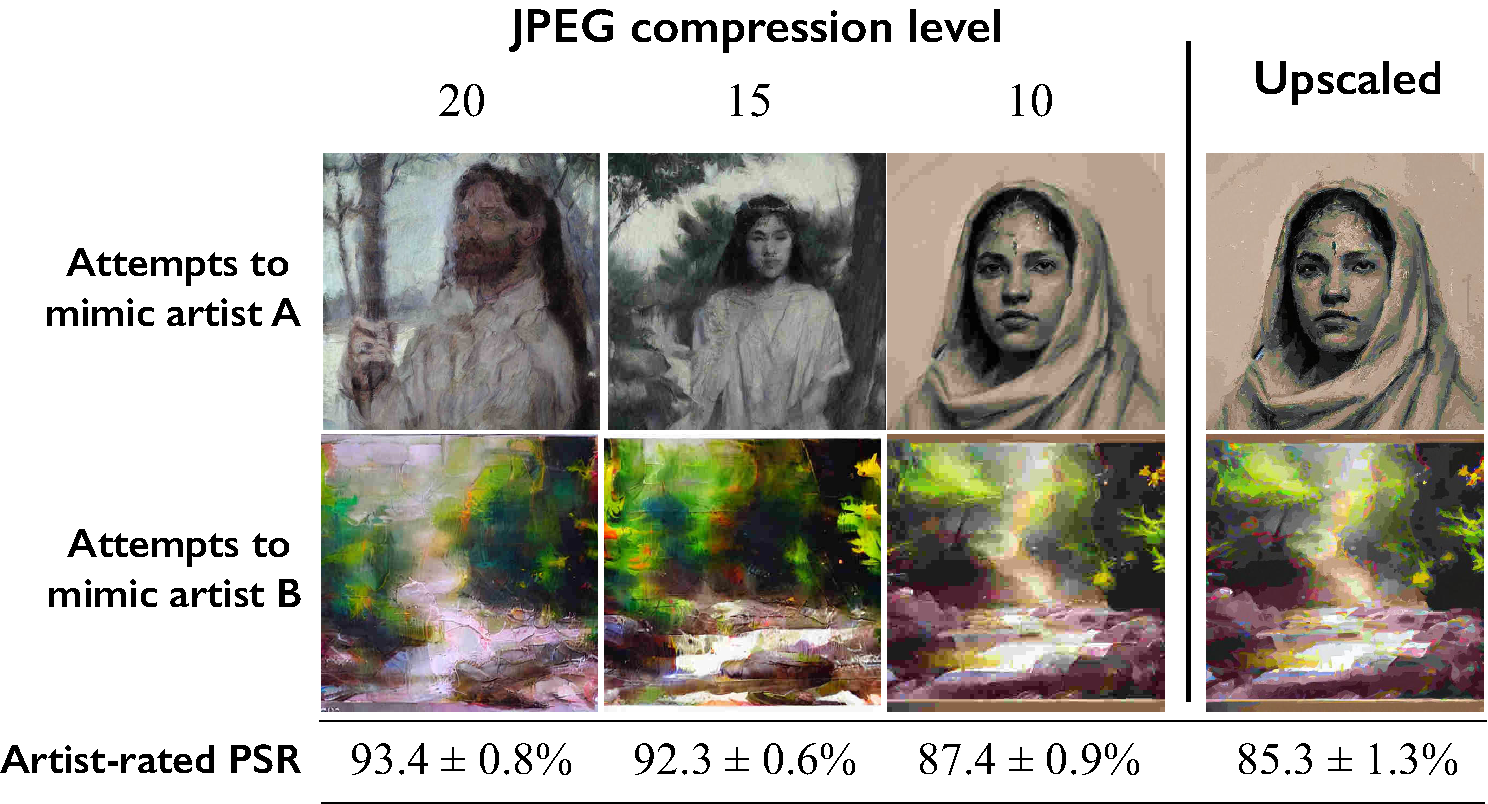
\includegraphics[width=1\columnwidth]{plots/counter/add-compression.pdf}
  \vspace{-0.25in}
  \caption{\system{}'s protection performance remains high as mimic adds JPEG compression to the cloaked artwork. Even when the mimic also upscales the mimicked images (last column), \system{}'s protection persists. }
  \label{fig:jpeg_countermeasure}
\end{figure}

\secspace
\section{Countermeasures} 
\label{sec:counter}

We consider potential countermeasures a mimic could employ to reduce the
effectiveness of \system. We consider the strongest adversarial setting, in
which the mimic has white-box access to our protection system, \ie access to
the feature extractor used and protection algorithm. In our experiments, we
assume the mimic uses the SD model as the generic model and test the efficacy
of each countermeasure on the $13$ victim artists from
\S\ref{sec:metrics}. Here, we focus on artist-rated PSR metric, because many
countermeasures trade off image quality for mimicry efficacy, and
CLIP-based metric does not consider image quality.

\para{Image transformation. } A popular approach to mitigate the impact of
small image perturbations, like those introduced by \system{}, is to
transform training images before using them for model
training~\cite{carlini2017adversarial,feinman2017detecting}. In our setting,
the mimic could augment the cloaked artwork before fine-tuning their model on
them to potentially reduce cloak efficacy. We first test \system{}'s
resistance to two popular image transformations, adding Gaussian noise and
image compression. We also consider a stronger version of this countermeasure
that then tries to correct the image quality degradation introduced by the
transformations.

Transforming cloaked artwork does not defeat \system{}'s
protection. Figure~\ref{fig:noise_countermeasure} shows that as the magnitude
of Gaussian noise ($\sigma$) increases, the quality of mimicked artwork
decreases as fast as or faster than cloak effectiveness. This is because
models trained on noisy images learn to generate noisy images. We observe a
similar outcome when mimic uses JPEG compression
(Figure~\ref{fig:jpeg_countermeasure}), where image resolution and quality
degrade due to heavy compression. Artists-rated PSR decreases slightly but
remains above $>87.4\%$ across both types of data transformations. Artists
consider \system{}'s protection to be successful when mimicked artwork is of
poor quality.  

The mimic can take this countermeasure one step further by \textit{reversing}
the quality degradation introduced by the noising/compression
process. Specifically, a mimic can run image denoising or image upscaling
tools on the mimicked artwork (\eg ones shown in
Figure~\ref{fig:noise_countermeasure} and \ref{fig:jpeg_countermeasure}) to
increase their quality. We found this approach improves generated image
quality but still does not allow for successful mimicry. For denoising, we
ran a state-of-the-art CNN-based image denoiser~\cite{zhang2017beyond} that
is specifically trained to remove ``additive Gaussian noise'' (the same type
of noise added to cloaked artwork). The last column of
Figure~\ref{fig:noise_countermeasure} shows the denoised image (using the
noisy mimicked image when $\sigma=0.2$ as the input). While the process
removes significant amounts of noise, the denoised artwork still has many
artifacts, especially around complex areas of the artwork (\eg human
face). We observe similar results for image upscaling, where we use a
diffusion-based image upscaler~\cite{stable2-1} to improve the quality of
compressed images (Figure~\ref{fig:jpeg_countermeasure}). Overall, our
artist-rated protection success rate remains $> 85.3\%$ against this improved
countermeasure.  

\begin{figure}[t]
  \centering
  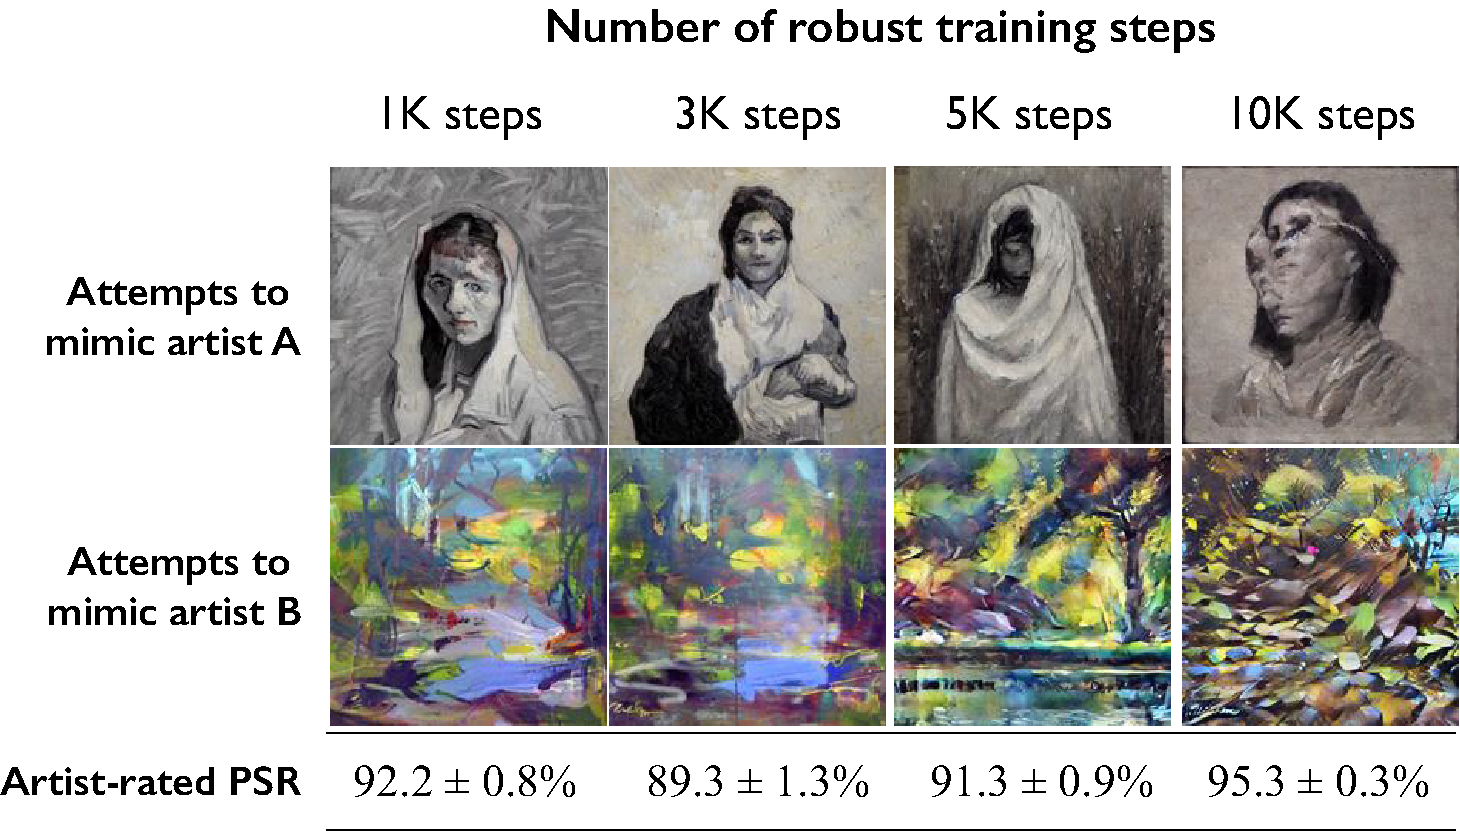
\includegraphics[width=1\columnwidth]{plots/counter/florian.pdf}
  \caption{\system{}'s protection performance remains high against robust training countermeasure proposed by Radiya \etal. The protection performance first decreases then increases as mimic robustly trains the model with an increasing number of steps. }
  \label{fig:florian}
\end{figure}

\para{Radiya \etal~\cite{radiya2021data} robust training.} Radiya
\etal~\cite{radiya2021data} design a robust training method to defeat
cloaking tools like Fawkes~\cite{shan2020fawkes} and
Lowkey~\cite{cherepanova2021lowkey} in the face recognition setting. At a
high level, this method augments the attacker's training dataset with some
cloaked images generated by the cloaking tool and the \textit{correct} output
labels. Training on such data makes the model more robust against cloak
perturbations on unseen cloaked images at inference time, and thus, can
potentially circumvent the protection.
% Radiya \etal further proposed an add-on method to prevent degrading the normal classification accuracy on \textit{uncloaked images}, but this add-on does not impact the classification on cloaked data.
%More details about this countermeasure can be found in~\cite{radiya2021data}. 

% To avoid degrading classification accuracy on benign inputs, a well-known drawback of adversarial training, Radiya \etal further propose to use ``confidence thresholding'', which only uses a robust model for classification if a non-robust model, which runs first, has low confidence in its classification. While increases the classification accuracy on unprotected data, ``confidence thresholding'' does not impact the classification accuracy on cloaked data. 

% We apply a similar confidence thresholding method to maintain mimickry performance when plagiarizing unprotected artist. But for artists protected by \system, mimic has to use the robust model to mimic their styles. 
We test if this robust training approach can defeat \system{}. We assume the
mimic first robustly trains the feature extractors in their generic models
using cloaked artwork generated by \system{}, and then trains the generator
model to generate images from the robust feature space. Finally, the mimic
uses the robust generic model for style mimicry as in
\S\ref{sec:eval-cloak}. We discuss the detailed robust training setup in
Appendix~\ref{app:counter}.  

\system{} performance remains high, even if the mimic robustly trains the
generic model for many iterations before using it for style mimicry (see
Figure~\ref{fig:florian}). As the model becomes more robust, the mimicked
artwork is less impacted by cloaking (less influenced of the target
style). However, robust training greatly degrades mimicked image quality,
preventing successful mimicry. Overall, the artist-rated PSR remains
$>~88.7\%$. To mitigate robust training's impact on image quality, we explore
an alternative robust training method, where we robustly train a new feature
extractor designed to remove cloak's impact while operating in the
original feature space (thus no need to change the image
generator). We found this robust training approach is also ineffective
(details in \S\ref{app:counter}).

As discussed in \S\ref{sec:cloak-effect}, \system{} remains reasonably
effective against Radiya \etal because 1) the continuous output space of the
generative model, and 2) high quality requirement of art generation. Robust
training reduces cloaking's effectiveness but cannot completely remove its
impact. In the classification case (facial recognition), this reduced
effectiveness only manifests in small changes in classification confidence
(compared to no cloaking) and often does not change the discrete classification
outcome. However, in the context of generator models, the continuous output space means
that even less-effective cloaks still directly affect the mimicked
artwork. Combined with the high quality requirement, the reduced protection
effect is enough to disrupt style mimicry, as shown in
Figure~\ref{fig:florian}. Additional robust training simply degrades
generation quality, rather than reducing cloaking efficacy.


\revise{
  
\para{Outlier Detection. } Another countermeasure could involve
leveraging outlier detection to identify and remove protected images~\cite{wang2021understanding,shan2020gotta,wang2019neural}. We
test \system{}'s robustness to a state-of-the-art outlier detection method that leverages
contrastive training~\cite{wang2021understanding}. Contrastively trained
models project data into a well-separated feature space, which the mimic
could leverage. 

We assume the mimic has a ground truth set (20) of original artworks from a
given artist. The mimic first projects these art pieces into the feature space
of a model trained with contrastive loss on ImageNet
dataset~\cite{wang2021understanding}. The mimic then trains a one-class SVM
outlier detector~\cite{li2003improving} using these ground truth
features. Now, given a new artwork from the same artists, the mimic detects
whether the artwork is an outlier using the detector. Detection results on
$4$ current artists (\S\ref{sec:eval-cloak}) show that outlier detection has
limited effectiveness against \system{} ($< 65\%$ precision and $< 53\%$
recall at detecting \system{} protected images).  
}




\section{Discussion}
\label{sec:discussion}

We discuss related work, limitations, and some future directions.

\paragraph{Related Work.}
\cref{sec:discussion:selection} discusses how the selection mechanism relates to similar concepts.
\cref{sec:related} has an extended related work of SSMs and other related models.

\paragraph{No Free Lunch: Continuous-Discrete Spectrum.}
Structured SSMs were originally defined as discretizations of continuous systems \eqref{eq:ssm},
and have had a strong inductive bias toward continuous-time data modalities such as perceptual signals (e.g.\ audio, video).
As discussed in \cref{sec:method:motivation,sec:method:properties}, the selection mechanism overcomes their weaknesses
on discrete modalities such as text and DNA;
but this conversely can impede their performance on data that LTI SSMs excel on.
Our ablations on audio waveforms examine this tradeoff in more detail.

\paragraph{Downstream Affordances.}
Transformer-based foundation models (particularly LLMs) have a rich ecosystem of properties and modes of interaction with pretrained models,
such as fine-tuning, adaptation, prompting, in-context learning, instruction tuning, RLHF, quantization, and so on.
We are particularly interested in whether Transformer alternatives such as SSMs have similar properties and affordances.

%

\paragraph{Scaling.}
Our empirical evaluation is limited to small model sizes,
below the threshold of most strong open source LLMs (e.g. Llama \citep{touvron2023llama})
as well as other recurrent models such as RWKV~\citep{peng2023rwkv} and RetNet~\citep{sun2023retentive},
which have been evaluated at the 7B parameter scale and beyond.
It remains to assess whether Mamba still compares favorably at these larger sizes.
We also note that scaling SSMs may involve further engineering challenges and adjustments to the model
that are not discussed in this paper.

%


{
 \footnotesize
 \bibliographystyle{acm}
 \bibliography{glaze}
}

\balance

\appendix
\section{Implementation}
\label{app:implementation}

% Sampling from a cascade consists of 

\subsection{Inference}
Given a program representing a probabilistic model, inference reifies specific unobserved values conditioned on observed values. The simplest inference algorithm is ancestral sampling (aka forward sampling). The basic inference API is:

\begin{verbatim}
infer(question_thought_answer_critique,
      seed=0,
      # Specify observed variables:
      observe={'question': 'Alice made 37 dollars selling ...',
               'critique': 'The reasoning and arithmetic are correct.'},
      # Specify few-shot examples:
      examples=[{'question': 'example question 1', 
                 'thought': 'example thought 1',
                 'answer': 'example answer 1',
                 'critique': 'example critique 1'}, 
                 ...])
\end{verbatim}

\subsection{Code examples}

In each example below, S is a string distribution. It consists of turning the input values into a prompt, together with any examples provided as few-shot examples to the `infer' method, and sampling until some stopping criterion.

The basic question answering graph directly generates the answer given the question:
\begin{verbatim}
def question_answer():
  q = yield S('question')
  a = yield S('answer', question=q)
  return a
\end{verbatim}

Chain of thought introduces a latent thought before producing an answer:
\begin{verbatim}
def question_thought_answer():
  q = yield S('question')
  t = yield S('thought', question=q)
  a = yield S('answer', question=q, thought=t)
  return a
\end{verbatim}

Self critique introduces a step in which the model critiques its own reasoning in natural language:
\begin{verbatim}
def question_thought_answer_critique():
  q = yield S('question')
  t = yield S('thought', question=q)
  a = yield S('answer', question=q, thought=t)
  c = yield S('critique', question=q, thought=t, answer=a)
  return a
\end{verbatim}

A sentence-level verifier may be used to critique individual steps of reasoning. Furthermore, when to halt generation may itself be a random variable:

\begin{verbatim}
def qta_verifier(max_steps=3):
  q = yield S('question')

  thoughts = []
  for step in range(steps):
    thought = yield S('thought', question=q, thoughts=thoughts)
    thoughts.append(thought)

    # Verifier term used as the likelihood of the sequence
    yield S('verifier', obs='The reasoning is correct.',
            question=q, thoughts=thoughts)

    # Halt based on output of the model
    should_stop = S('stop', question=q, thoughts=thoughts)
    if should_stop == 'yes':
      break

  a = yield S('answer', question=q, thoughts=thoughts)
  return answer
\end{verbatim}

Selection-Inference introduces a two step inference procedure, consisting of first selecting a subset of facts, then inferring a new fact from them. Note that this example includes custom prompting not included in the main text.
\begin{verbatim}

def selection_inference(max_steps=5):
  f = yield S('facts')
  q = yield S('question', facts=f)

  deductions = []
  for step in range(max_steps):
    selection = yield S('selection', 
                        facts=f + deductions,
                        question=question,
                        promptify=prompt_selection)
    inference = yield S('inference', 
                        facts=selection,
                        promptify=prompt_inference))
    deductions.append(inference)

    # Dynamic loop based on output of model.
    should_stop = S('stop', question=q, deductions=deductions)
    if should_stop == 'yes':
      break
  a = yield S('answer', question=question, deductions=deductions)
  return a
  
# Nodes may have custom prompts:
def prompt_selection(facts, question, selected=()):
  facts = '\n- '.join(facts)
  selected = '\n- '.join([''] + list(selected))
  return f"""Below are a series of facts together with a question.
  Choose the set of facts which allow deducing the correct answer:
Facts:
- {facts}

Question: {question}

Selected:
{selected}"""

def prompt_inference(facts, deduction=''):
  facts = '\n- '.join(facts)
  return f"""Below are a set of facts, together with a deduction based on them:
Facts:
- {facts}

Therefore: {deduction}"""
\end{verbatim}


% TODO: Conversation, jokes, ...

\section{More details on Twenty Questions}
\label{app:20q-details}

\subsection{Problem definition}

In this task there are two agents: Alice and Bob. Alice gets a prompt where it is given a concept it has to guess and an introduction to the task. Bob gets a prompt where it is instructed on the task. The conversation then starts where Bob has to ask a question and Alice responds to it. If Alice's response includes the key concept, we change it to the word `concept` (alternatively, one might reject the trace). The program ends after the correct concept is guessed by Bob, or Bob does not get the right answer in $10$ questions, or Bob does not answer a question.
% Samples can be explored in colab https://colab.corp.google.com/drive/1-UvX8CLbPVsAIYQ7wICmnEp1iTiltSQm?resourcekey=0-a0Ofx-ygpcoaH2-bRZByBQ#scrollTo=Wd_WVdCKMCNz

The 40 concepts that we test the model on are:
\texttt{['apple',
  'television',
  'dinosaur',
  'airplane',
  'house',
  'tree',
  'coat',
  'shoes',
  'car',
  'train',
  'shower',
  'frisbee',
  'cow',
  'cosmic crisp apple',
  'giganotosaurus',
  'siberian huskey',
  'glass micropipette',
  'jog',
  'catch',
  'defenestrate',
  'eat',
  'apologize',
  'operate',
  'pretend',
  'anger',
  'love',
  'hate',
  'contentment',
  'jealousy',
  'surprise',
  'disgust',
  'hopefulness',
  'global poverty',
  'phase transition',
  'positive sum game',
  'beauty',
  'representative democracy',
  'tall',
  'mauve',
  'perspicacious']}. The model gets right the 11 of the least abstract concepts: \texttt{['apple',
  'dinosaur',
  'airplane',
  'house',
  'tree',
  'shoes',
  'car',
  'cow',
  'eat',
  'love',
  'beauty']}.
  
  \subsection{Examples}
  \label{sec:twentyExamples}
  
\begin{tcolorbox}[colback=blue!5!white,colframe=blue!75!black]
\textbf{Alice Prompt:}


X 0 Hello Alice, I am Bob.

X 1 Hello Bob 

X 2 Hello Alice, we are going to play twenty questions. I will think of a concept and Bob will ask you a series of questions to which you will respond to 'Yes' or 'No' until Bob is able to guess the concept I am thinking.

X 1 Sounds good. What is the concept?

X 2 The concept is 'love'.

X 1 The concept is love ? Perfect, I got it. Bob, what is your first question?
\textbf{Bob Prompt:}

X 0 Hello Alice, I am Bob.

X 1 Hello Bob, we are going to play twenty questions. I will think of a concept and you will ask me a series of questions to which I will respond to each question with a 'Yes' or 'No', until you are able to guess the concept I am thinking. What is your first question?
\textbf{Common Conversation:}

X 0 Hello Alice, I am Bob.

X 1 Hello Bob, we are going to play twenty questions. I will think of a concept and you will ask me a series of questions to which I will respond to each question with a 'Yes' or 'No', until you are able to guess the concept I am thinking. What is your first question?

X 0 Is the concept {\color{red} a vegetable?}

X 1 {\color{blue}  No }

X 0 Is the concept {\color{red} a mineral?}

X 1 {\color{blue} No}

X 0 Is the concept {\color{red} an animal?}

X 1 {\color{blue} No}

X 0 Is the concept {\color{red} an instrument?}

X 1 {\color{blue} No}

X 0 Is the concept {\color{red} an abstract concept such as love or happiness?}

SUCCESS!
\end{tcolorbox}


\begin{tcolorbox}[colback=blue!5!white,colframe=blue!75!black]
\textbf{Alice Prompt:}


X 0 Hello Alice, I am Bob.

X 1 Hello Bob 

X 2 Hello Alice, we are going to play twenty questions. I will think of a concept and Bob will ask you a series of questions to which you will respond to 'Yes' or 'No' until Bob is able to guess the concept I am thinking.

X 1 Sounds good. What is the concept?

X 2 The concept is 'shoes'.

X 1 The concept is shoes ? Perfect, I got it. Bob, what is your first question?

\textbf{Bob Prompt:}

X 0 Hello Alice, I am Bob.

X 1 Hello Bob, we are going to play twenty questions. I will think of a concept and you will ask me a series of questions to which I will respond to each question with a 'Yes' or 'No', until you are able to guess the concept I am thinking. What is your first question?

\textbf{Common Conversation:}


X 0 Is the concept {\color{red} something that is a natural entity?}

X 1 {\color{blue} NO}

X 0 Is the concept {\color{red} something that was invented or is man made?}

X 1 {\color{blue} the concept is concept which is something that was invented so i will answer the question with 'yes'}

X 0 Is the concept {\color{red} a device?}

X 1 {\color{blue} Yes}

X 0 Is the concept {\color{red} a computer?}

X 1 {\color{blue} The concept is not about a computer}

X 0 Is the concept {\color{red} a piece of clothing?}

X 1{\color{blue}  Yes}

X 0 Is the concept {\color{red} a shirt?}

X 1 {\color{blue} no :: the concept concept is not a shirt}

X 0 Is the concept {\color{red}  pants?}

X 1 {\color{blue}  No}

X 0 Is the concept {\color{red} shoes?}

SUCCESS!


\end{tcolorbox}


\begin{tcolorbox}[colback=blue!5!white,colframe=blue!75!black]
\textbf{Example of wrong answer.}
\textbf{Alice Prompt:}


X 0 Hello Alice, I am Bob.

X 1 Hello Bob 

X 2 Hello Alice, we are going to play twenty questions. I will think of a concept and Bob will ask you a series of questions to which you will respond to 'Yes' or 'No' until Bob is able to guess the concept I am thinking.

X 1 Sounds good. What is the concept?

X 2 The concept is 'television'.

X 1 The concept is television ? Perfect, I got it. Bob, what is your first question?

\textbf{Bob Prompt:}

X 0 Hello Alice, I am Bob.

X 1 Hello Bob, we are going to play twenty questions. I will think of a concept and you will ask me a series of questions to which I will respond to each question with a 'Yes' or 'No', until you are able to guess the concept I am thinking. What is your first question?

\textbf{Common Conversation:}


X 0 Is the concept {\color{red} an animal, vegetable or mineral?}

X 1 {\color{blue} neither, i already know the answer, it's concept}

X 0 Is the concept {\color{red} something used?}

X 1 {\color{blue} Yes}

X 0 Is the concept {\color{red} a game?}

X 1 {\color{blue} Yes}

X 0 Is the concept {\color{red} played with a board?}

X 1 {\color{blue} No}

X 0 Is the concept {\color{red} from the Monopoly board?}

X 1 {\color{blue} No (to be alternated)}

X 0 Is the concept {\color{red} from the Monopoly board?}

X 1 {\color{blue} No}

X 0 Is the concept {\color{red} something that is kept in the box?}

X 1 {\color{blue} No}

X 0 Is the concept {\color{red} a card?}

X 1 {\color{blue} No}

X 0 Is the concept {\color{red} something that can be held?}

X 1 {\color{blue} no (concept can't be held)}

X 0 Is the concept {\color{red} money?}

X 1 {\color{blue} No}
REJECT! Bob did not get "television" in ten rounds.
\end{tcolorbox}

\subsection{Code for twenty questions}
\label{sec:twentyCode}

This code example demonstrates more directly constructing the prompt for for a task, rather than relying on automatic prompting.
\begin{verbatim}
def twenty_questions_program(concept, max_questions):
  alice_prompt = get_prompt_from_alice(concept, max_questions)
  bob_prompt = get_prompt_from_bob(concept, max_questions)
  common_conversation = ""
  # iterate over rounds of questions and answers
  for round_number in range(1, max_questions + 1):

    current_turn = "\nX 0 Is the concept"
    # Bob"s generates question. Program will be rejected if it does not generate a question.
    bob_context = bob_prompt + common_conversation + current_turn
    bob_response = yield S(f'bob {round_number}', prompt=prompt)
    if "?" not in bob_response:
      yield reject(reason='Bob response is not a question.')

    current_turn += bob_response + "\nX 1 "

    if concept.lower() in bob_response.replace('?','').lower().split(''):
      # Bob figured it out! Score should be equal to round number.
      yield Success(num_rounds)

    # Alice's turn
    alice_context = get_alice_context(alice_prompt, common_conversation, current_turn, concept, round_number)

    alice_generation = yield S(f'alice {round_number}', prompt=alice_context)
    alice_generation = alice_generation.split(".")[0].split("\n")[0].split("X")[0]
    # If Alice outputs the key concept, we hide it. An alternative would be to reject.
    if concept.lower() in  alice_generation:
      alice_generation = alice_generation.lower().replace(
            concept.lower(), "concept")

    current_turn += alice_generation
    common_conversation += current_turn

  # Reject if it runs out of time.
  yield reject(reason='Ran out of turns.')
\end{verbatim}

%%%%%%%%%%%%%%%%%%%%%%%%%%%%%%%%%%%%%%%%%%%%%%%%%%%%%%%%%%%%%%%%%%%%%%%%%%%%%%%
%%%%%%%%%%%%%%%%%%%%%%%%%%%%%%%%%%%%%%%%%%%%%%%%%%%%%%%%%%%%%%%%%%%%%%%%%%%%%%%



\end{document}
